\documentclass[11pt]{article}
\usepackage{amsfonts,amsmath,amssymb,amsthm}
\usepackage{graphicx,psfrag,epsf}
\usepackage{enumerate}
\usepackage{url} % not crucial - just used below for the URL 
\usepackage{algorithm}
\usepackage{algpseudocode}
\usepackage{subfig}
\usepackage{authblk}
\usepackage{verbatim} %used to comment out unnecessary contents
\usepackage{helvet}
\usepackage[colorlinks=true,pagebackref,linkcolor=magenta]{hyperref}
\usepackage[sort&compress,comma,square,numbers]{natbib}
\usepackage{fullpage,fancyhdr}
\renewcommand{\familydefault}{\sfdefault}
\usepackage{color} %used to highlight changes
\usepackage{paralist}

\pagestyle{fancy}
% \oddsidemargin=-0.5in 
% \evensidemargin=-0.5in
\textwidth=6.5in 
\headwidth=6.5in
\textheight=9.0in 
\headheight=0.0pt
\topmargin=0.0in
\headsep=0.0in
\renewcommand{\headrulewidth}{0pt}

\setlength{\parindent}{0em}
\setlength{\parskip}{0.5em}

% % DON'T change margins - should be 1 inch all around.
% \addtolength{\oddsidemargin}{-.5in}%
% \addtolength{\evensidemargin}{-.5in}%
% \addtolength{\textwidth}{1in}%
% \addtolength{\textheight}{-.3in}%
% \addtolength{\topmargin}{-.8in}%


\providecommand{\sct}[1]{{\sc \texttt{#1}}}
\providecommand{\mt}[1]{\widetilde{#1}}
\providecommand{\mb}[1]{\boldsymbol{#1}}
\providecommand{\mc}[1]{\mathcal{#1}}
\newcommand{\Real}{\mathbb{R}}
\newcommand{\G}{\mathcal{G}}
\newcommand{\K}{\mathcal{K}}
\newcommand{\LL}{\mathcal{L}}
\newcommand{\Migraine}{\sct{Migraine}}
\newcommand{\mtg}{\sct{m2g}}
\newcommand{\T}{^{\ensuremath{\mathsf{T}}}}           % transpose
\newcommand{\Linefor}[2]{%
    \State \algorithmicfor\ {#1}\ \algorithmicdo\ {#2} \algorithmicend\ \algorithmicfor%
}
\newcommand{\subfigimg}[3][,]{%
  \setbox1=\hbox{\includegraphics[#1]{#3}}% Store image in box
  \leavevmode\rlap{\usebox1}% Print image
  \rlap{\hspace*{12pt}\raisebox{\dimexpr\ht1-0\baselineskip}{#2}}% Print label
  \phantom{\usebox1}% Insert appropriate spcing
}

%environment
\newtheorem{thm}{Theorem}
\newtheorem{appThm}{Theorem}
\setcounter{appThm}{0}
\newtheorem{lem}{Lemma}
\newtheorem{cor}{Corollary}
\newtheorem*{defi*}{Properties}
\newtheorem{asn}{Assumption}
\newcommand*\mean[1]{\bar{#1}}
\begin{document}

\def\spacingset#1{\renewcommand{\baselinestretch}%
{#1}\small\normalsize} \spacingset{1}

\title{\bf Dependence Discovery from Multimodal Data via  Multiscale Graph Correlation}
\author[1]{Cencheng Shen\thanks{cshen@temple.edu}}
\author[2]{Carey E. Priebe\thanks{cep@jhu.edu}}
\author[3]{Mauro Maggioni\thanks{mauro.maggioni@duke.edu}}
\author[4]{Joshua T. Vogelstein\thanks{jovo@jhu.edu}}
\affil[1]{Department of Statistics, Temple University}
\affil[2]{Department of Applied Mathematics and Statistics, Johns Hopkins University}
\affil[2]{Department of Mathematics, Duke University}
\affil[4]{Department of Biomedical Engineering and Institute for Computational Medicine, Johns Hopkins University}
\maketitle
\pagestyle{empty}

\bigskip
\begin{abstract}
Understanding and discovering dependence between multiple properties or measurements of our world is a fundamental task not just in science, but also policy, commerce, and other domains. 
%In the past hundred years, people have developed many different measures of dependence that can be applied in a wide variety of settings.  
In this paper we propose a novel dependence test statistic called ``Multiscale Graph Correlation'' (MGC), having the following properties: (1) Theoretical consistency such that the testing power converges to $1$ under any dependency structure and dimensionality. 
%Strong theoretical support, guaranteeing rejecting independence no matter what the dependence structure is, and failing to reject when no dependence is present. 
(2) Strong empirical performance on a wide variety of low- and high-dimensional simulations. (3) Provides insight into the local scales in which dependency is strongest. (4) On real data, detects dependence when it exists, and does not inflate the false positive rate in the absence of dependency. 
%No existing test satisfies all of these properties. 
Briefly, we combine the ideas of distance correlation with nearest-neighbor testing to develop MGC, and demonstrate its properties and advantages by extensive theory, simulations, and real data examples. We can therefore use MGC and local correlation coefficients in a variety of settings in which previous tests failed to detect signal or provide insight.
\end{abstract}

\noindent%
{\it Keywords: testing independence, distance correlation, k-nearest-neighbor, local correlation coefficient, permutation test}
\vfill

\clearpage
\tableofcontents

% science report: 2500 words
% science article: 4500 words

\newpage
\spacingset{1.45}

\section{Introduction}
\label{sec:intro}
With the increasing type, size, and dimension of modern data sets, detecting dependency among multiple data sets is one of the most important and fundamental tasks in the big data age. The Pearson's correlation coefficient \cite{Pearson1895}, Spearman's and Kendall's rank correlation coefficient \cite{KendallBook}, RV coefficient \cite{RobertEscoufier1976}, Procrustes coefficient \cite{GowerProcrustesBook}, information theoretic measures \cite{Renyi1959}, and the Mantel test \cite{Mantel1967} have been the traditional tools for this task, but each has its limitations when dealing with the increasingly complex modern data sets, e.g., the Pearson's correlation coefficient and RV coefficient are mostly useful for finding linear relationship and may be zero for nonlinear dependent data sets, while mutual information performs poorly for high-dimensional data. 

Many recent methods have been proposed to identify the existence of potential relationships between data sets, including \cite{Baringhaus2004,TaskinenOjaRandles2005, GrettonEtAl2005, SzekelyRizzoBakirov2007, GrettonGyorfi2010,Reshef2011, HellerGorfine2013, Reimherr2013, SzekelyRizzo2013a, SzekelyRizzo2013b, RizzoSzekely2016,HHG2016}, etc. In particular, the distance correlation method from \cite{SzekelyRizzoBakirov2007, SzekelyRizzo2009, SzekelyRizzo2013a, SzekelyRizzo2014} has gained much popularity in the statistical community, due to its theoretical soundness and good numerical performance in testing independence. A similar method from the machine learning community is the kernel-based independence test, which is developed in \cite{GrettonEtAl2005, GrettonGyorfi2010, GrettonEtAl2012} and closely related to the distance-based method \cite{SejdinovicEtAl2013, RamdasEtAl2015}.

Despite current progress in the area, it remains a difficult problem to test dependency in practice; and even the best method in theory may suffer from one or more challenges underlying the modern data, such as small or huge sample size, high dimensionality, nonlinearity, noise, etc. For example, although distance correlation is consistent against all dependent alternatives when testing on Euclidean data, the sample distance correlation (dcorr) under-performs in many nonlinear or high-dimensional dependencies during finite-sample testing. The modified distance correlation (mcorr) from \cite{SzekelyRizzo2013a} adjusts the high-dimensional bias, but is still sub-optimal for many common nonlinear dependencies. In comparison, the HHG statistic developed in \cite{HellerGorfine2013} performs much better on nonlinear data of small sample size, but loses some testing power under certain noisy or high-dimensional dependencies. 

In a complementary literature, nearest-neighbor graphs have been used as a key computational primitive in many statistical tasks, ranging from classification and regression \cite{Stone1977} to data compression to recommender systems \cite{Sarwar2000}. Moreover, it has become an invaluable tool in unfolding nonlinear geometry in many recent development of nonlinear embedding algorithms, including Isomap \cite{TenenbaumSilvaLangford2000, SilvaTenenbaum2003}, Local Linear Embedding \cite{SaulRoweis2000, RoweisSaul2003}, and Laplacien eigenmaps \cite{BelkinNiyogi2003}, among many others; and a good choice of joint neighborhood can better unfold the nonlinearity and match data sets of multiple modality \cite{ShenVogelsteinPriebe2016}.

Most relevant to our work, a number of approaches to two-sample and dependence testing have utilized nearest-neighbor graphs \cite{David1966,Friedman1983,Schilling1986,Dumcke2014}.  These approaches have the advantage of naturally operating on any kind of data, including categorical and structured data, as well as strong theoretical guarantees.  Perhaps more importantly, they focus only on local distances, rather than global distances, enabling them to be robust to nonlinear and high-dimensional dependence structures.  However, these existing graph based tests do not provide a convenient or automatic way to choose the appropriate neighborhood size, therefore leaving a crucial tuning parameter unspecified, and greatly impairs their practical usages and finite sample performances. 

In this paper, we propose Multiscale Graph Correlation (MGC) to better address those challenges from modern data analysis. By marrying ideas from the distance correlation literature to those from the nearest neighbor literature, and adding some of our own special sauce, we obtain a test better than those in either camp.  More specifically,  the multiscale test is able to efficiently compute all local correlation coefficients to locate the optimal local scale, naturally inherits the advantages of the respective global correlation such as the consistency of dcorr, enjoys the properties of graph dependence structures such as better testing powers under nonlinear and high-dimensional dependencies, and is a scalable method on big data. 

These advantages make our new test statistic a great method for dependency discovery on complex simulated dependencies and real data. Indeed, in a comprehensive simulation setting, MGC is able to achieve superior finite-sample testing powers for data sets of nonlinearity, high-dimensionality, noise, and small sample size, comparing to existing popular methods like dcorr / mcorr / Mantel / HHG; and in the real data experiment, we show that MGC is able to uncover the underlying dependency when testing between related data sets,  and does not inflate the false positive rate when the dependencies are not there in a set of brain imaging experiments. Thus, we expect MGC and the notion of local correlation coefficients to find values in a wide range of applications.  To facilitate this, we provide open source MATLAB and R implementations of MGC, and incorporate into FlashR.

\section{Results}
\label{main}
\subsection{Description of Multiscale Graph Correlation}
\label{main1}
There are two key insights from the literature that we combine to develop our methodology.  First, a collection of pairwise comparisons  suffices to characterize a joint distribution \cite{Maa1996}.  Second, nonlinear manifolds can be approximated by local linear spaces.  Combining these two ideas yields the notion of local correlation coefficient, and we name the optimal local correlation as Multiscale Graph Correlation (MGC).  

Perhaps the first realization that pairwise properties can characterize a joint distribution comes from  Karl Pearson, who created Pearson's Product-Moment Correlation \cite{Pearson1895} by letting $a_{ij}=x_i$ and $b_{ij}=y_i$ in the following general form:
\begin{equation}
\label{generalCoef}
\G=\frac{\sum_{i,j=1}^n (a_{ij}-\bar{a}) (b_{ij}-\bar{b})}{\sqrt{\sum_{i,j=1}^n  (a_{ij}-\bar{a})^{2} \sum_{i,j=1}^n (b_{ij}-\bar{b})^{2}}}, 
\end{equation}

where $\bar{a}$ and $\bar{b}$ denote the sample means of $a_{ij}$ and $b_{ij}$. Equation~\ref{generalCoef} represents a generalized correlation coefficient, which characterizes most correlation coefficients since then.  For example, Spearman and Kendall's rank correlations set $a_{ij}$ to be $rank(x_i)-rank(x_j)$ and $sign(x_i-x_j)$ respectively \cite{KendallBook}; the Mantel coefficient \cite{Mantel1967} considers distance matrices and takes $a_{ij}=|x_i-x_j|_{2}$, which has been a popular method in biology and ecology. More recently, Szekely et al. \cite{SzekelyRizzoBakirov2007} proves that by doubly centering the distance matrices and using the resulting centered distance entries as $a_{ij}$, the ``distance correlation'' statistic is a consistent test for independence --- a test whose power approaches $1$ as sample size approaches infinity, for any joint distribution of finite dimension and finite second moments; and by further adjusting the properly centered distance entries, the modified distance correlation is consistent as the dimensionality of $x_{i}$ and $y_{i}$ approach infinity \cite{SzekelyRizzo2013a}. This is in contrast to other correlation coefficients including Pearson / rank / Mantel, which do not have theoretical consistency against all dependent alternatives. However, as all sample data are required to compute those correlations, the resulting coefficients may suffer from non-linearity / noise / outliers in the inference task.

In a separate academic lineage, manifolds have take center stage.  A manifold is a topological space that can be approximated by a collection of local flat Euclidean spaces.  Although nonlinear manifold learning has been around since at least the 1950s \cite{TorgersonBook}, it rose to prominence in the early 2000s when Local Linear Embedding \cite{SaulRoweis2000} and Isomap \cite{TenenbaumSilvaLangford2000} popularized the notion that computing distances between neighboring points could enable ``unfolding'' the manifold to discover its structure.  Since then, a multitude of theoretical and empirical studies have devised different nonlinear dimensionality reduction techniques \cite{LeeVerleysen2007}, most of which are essentially generalized principal components analysis \cite{ScholkopfSmolaMuller1999}.  These approaches all require choosing the neighborhood size, a parameter of paramount importance for subsequent inference. Despite of many efforts to numerically determine the parameter, to our knowledge, no approach provides a theoretically justified method for choosing the neighborhood. From a statistical point of view, the multiscale graph structure is useful for testing purposes \cite{David1966,Friedman1983,Schilling1986,Dumcke2014,HHG2016}, where choosing the appropriate local scale is also a difficult and time-consuming task. 

Our Multiscale Graph Correlation (MGC) combines generalized correlation coefficients with multiscale graph distances, in an effort to efficiently uncover local relationships and optimize the independence test.  Specifically, let $rank(a_{ij})$  be the ``rank'' of $x_i$ relative to $x_j$, that is, $rank(a_{ij})=k$ if $x_i$ is the $k^{th}$ closest point (or ``neighbor'') to $x_j$; and the ranks start from $k=1$ onwards (i.e., $rank(a_{jj})=1$), and the minimal rank is used for ties.  Then for any general correlation coefficient $\G$ in the form of Equation~\ref{generalCoef}, we define its \emph{local} variants by
\begin{equation}
\label{localCoef}
\G_{kl}=\frac{\sum_{i,j=1}^n (a_{ij}^k-\bar{a}^{k}) (b_{ij}^l-\bar{b}^{l})}{\sqrt{\sum_{i,j=1}^n  (a_{ij}^{k}-\bar{a}^{k})^2 \sum_{i,j=1}^n (b_{ij}^{l}-\bar{b}^{l})^2}},
\end{equation}
for $k=1,\ldots,\max(rank(a_{ij}))$, $l=1,\ldots,\max(rank(b_{ij}))$, where
\begin{equation}
\label{localCoef2}
    a_{ij}^k=
    \begin{cases}
      a_{ij}, & \text{if } rank(a_{ij}) \leq k, \\
      0, & \text{otherwise};
    \end{cases} \qquad \qquad
    b_{ij}^l=
    \begin{cases}
      b_{ij}, & \text{if } rank(b_{ij}) \leq l, \\
      0, & \text{otherwise};
    \end{cases}
\end{equation}
and $\bar{a}^{k}$ and $\bar{b}^{l}$ are the sample means of $a_{ij}^{k}$ and $b_{ij}^{l}$. For example, $\G_{kl}$ can be a local Pearson's / rank / Mantel / dcorr / mcorr correlation by plugging in the respective $a_{ij}$ and $b_{ij}$ from the corresponding global correlation coefficient $\G$; and there are a total of $\max(rank(a_{ij})) \times \max(rank(a_{ij}))$ local correlations, which equals $n^2$ when there exists no repeating point in the data.

\begin{figure}[htbp]
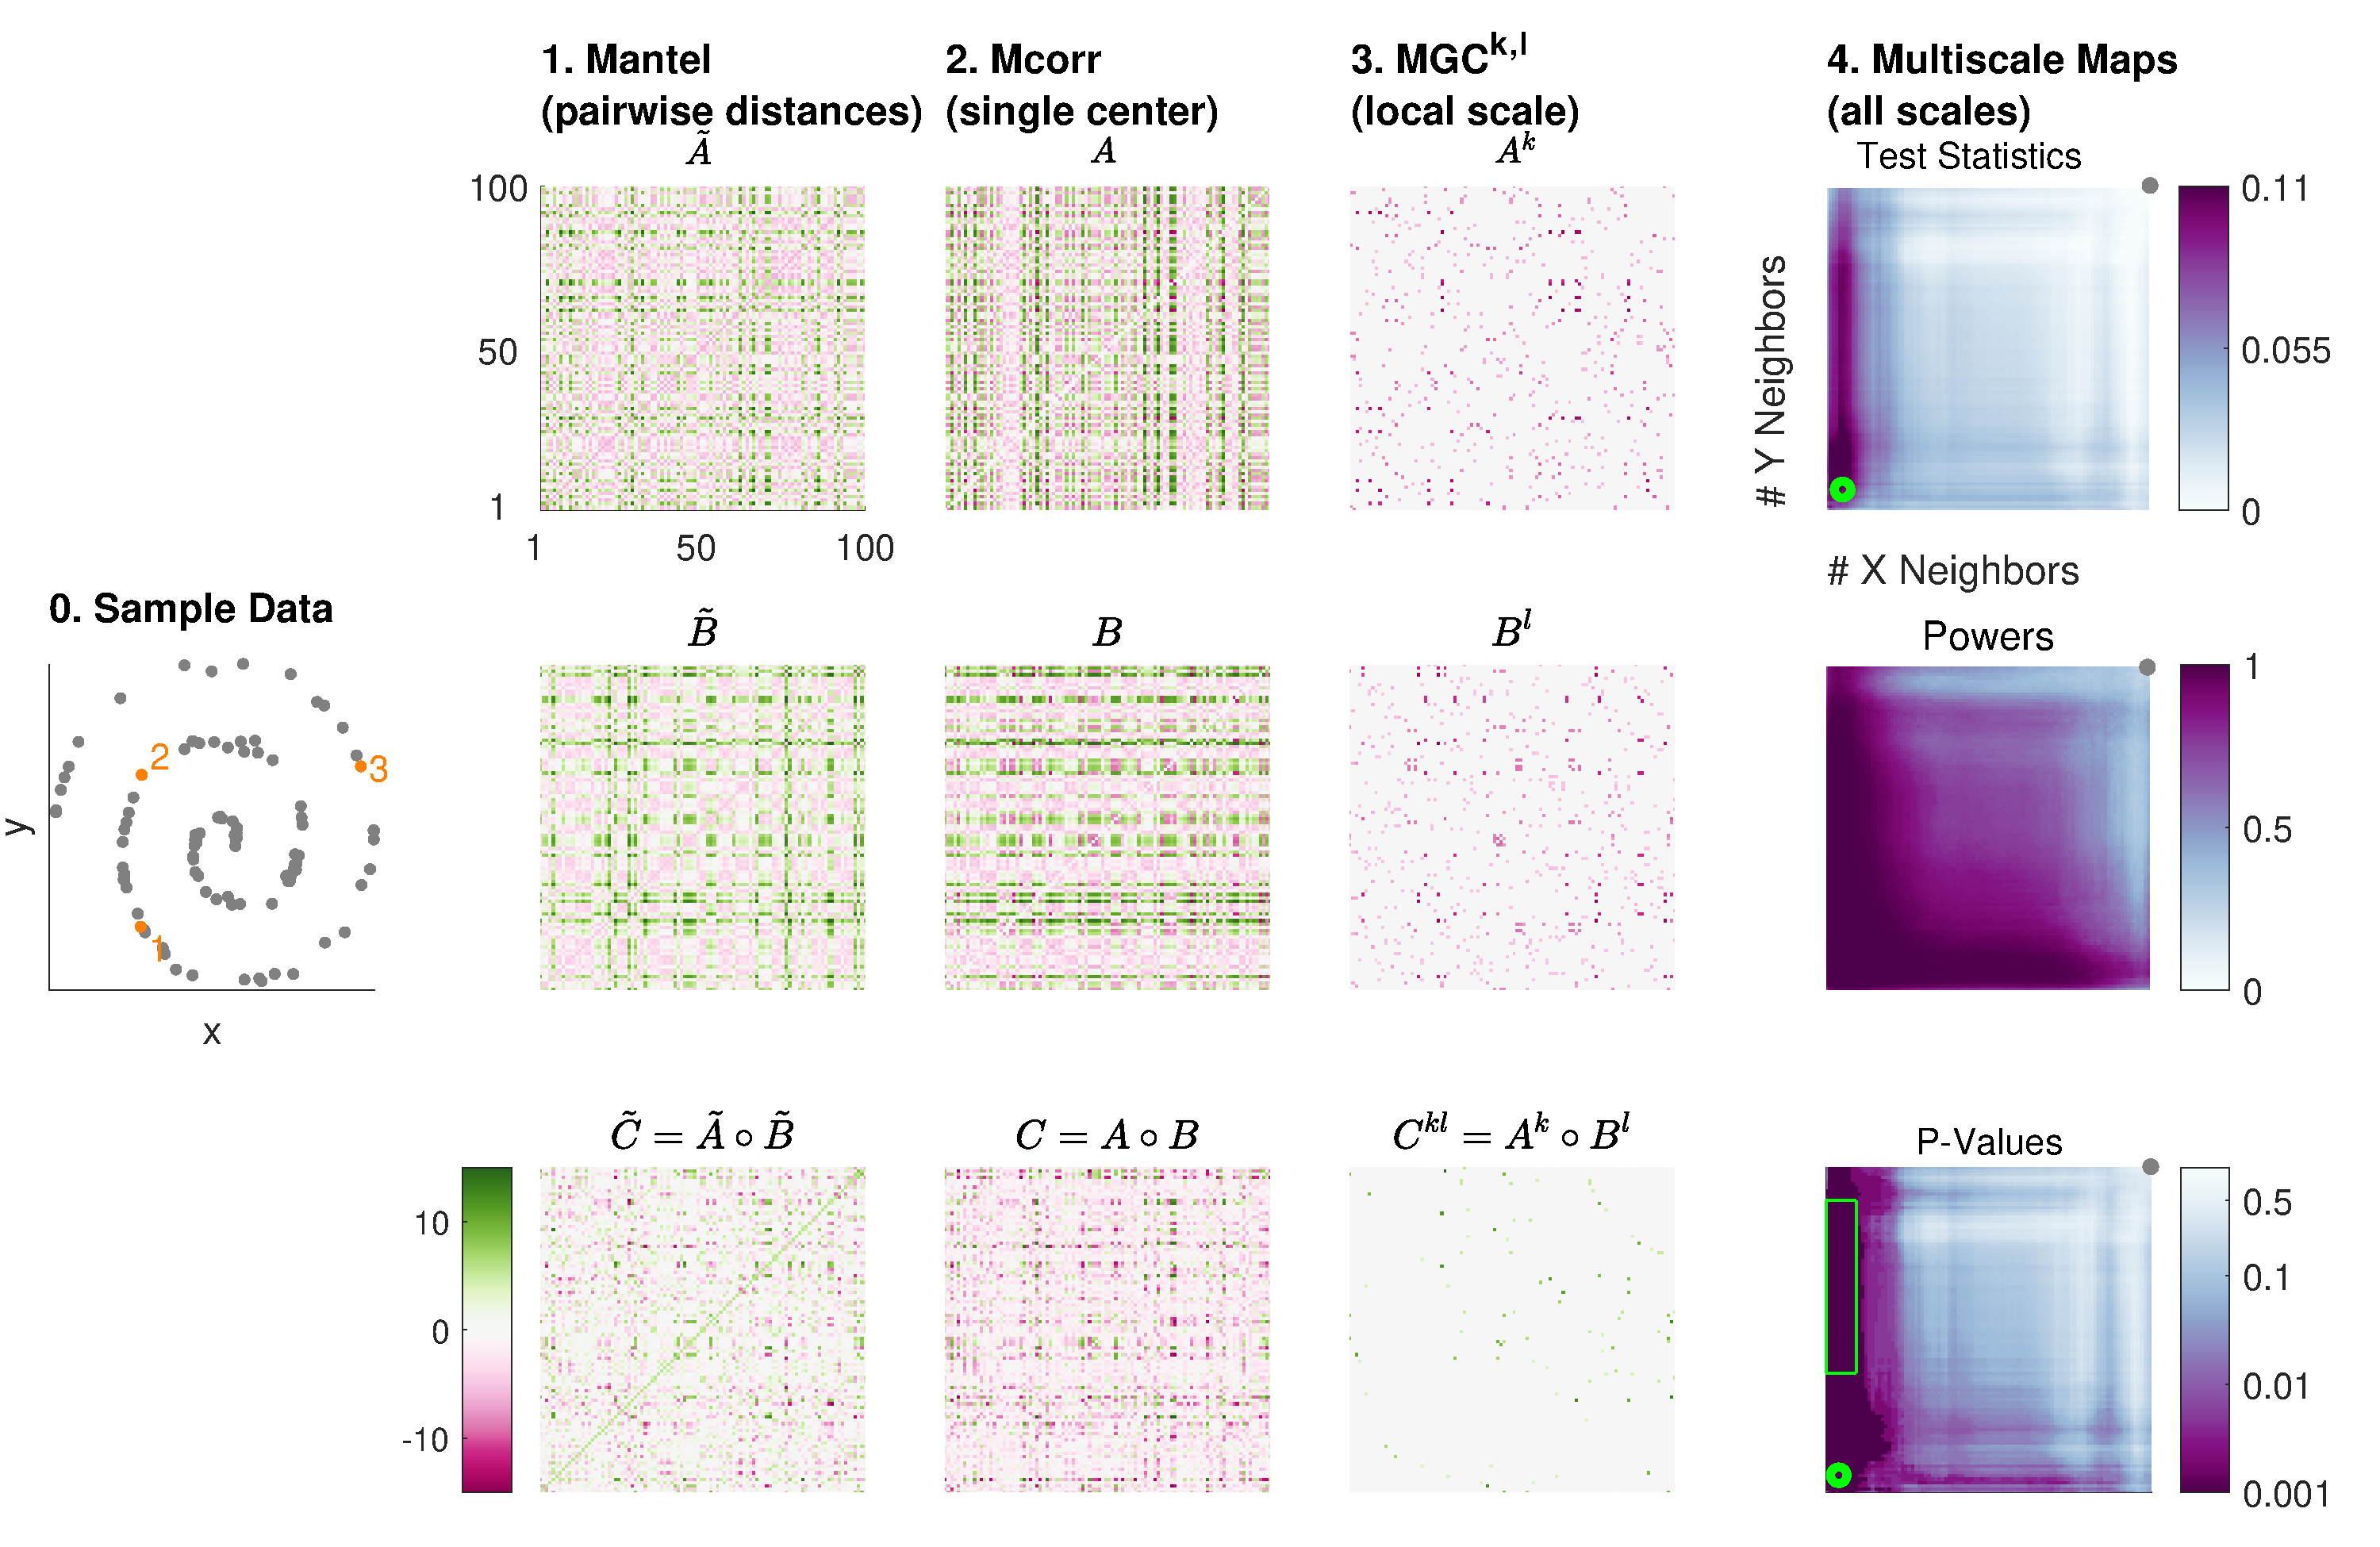
\includegraphics[width=1.0\textwidth]{Figures/FigA}
\caption{
Flowchart for local correlation computation: Column 1: $(X,Y)$ have a quadratic relationship with white noise. Column 2: The heat maps of $\tilde{A}$ and $\tilde{B}$, which are the pairwise Euclidean distance matrices of $X$ and $Y$. Column 3: The heat maps of $A=\{a_{ij}\}$ and $B=\{b_{ij}\}$, which are the normalized (i.e. doubly centered) distance matrices of $\tilde{A}$ and $\tilde{B}$. Column 4: The heat maps of local $A$ and $B$, i.e., $A^{k^{*}}=\{a^{k^{*}}_{ij}\}$ and $B^{l^{*}}=\{b^{l^{*}}_{ij}\}$, where $(k^{*},l^{*})$ is the optimal scale for the quadratic relationship. Column 5: The heat map of the entry-wise product of local $A$ and $B$, i.e., $\{(a_{ij}^{k^{*}}-\bar{a}^{k^{*}}) (b_{ij}^{l^{*}}-\bar{b}^{l^{*}})\}$ for $i,j=1,\ldots,n$. The matrix sum $\sum_{i,j}(a_{ij}^{k^{*}}-\bar{a}^{k^{*}}) (b_{ij}^{l^{*}}-\bar{b}^{l^{*}})$ equals the optimal local covariance, i.e., the un-normalized MGC statistic $\G^{*}$. }
\label{fig:A}
\end{figure}

In the family of local statistics $\{\G_{kl}\}$, the optimal local correlation coefficient (optimal with respect to the independence testing power) is dubbed the multiscale graph correlation and denoted as $\G^{*}$. Clearly the optimal scale exists, is distribution dependent, and may not be unique. But different from a manifold learning task, once the rank information is given, all local correlation coefficients can be simultaneously computed in the same running time complexity as the global correlation coefficient, which allows our definition of local correlations to be an efficient and general tool in data analysis.

Under the dependence testing framework, the optimal scale for MGC can be easily determined: if the underlying joint distribution is known, or multiple dependent data are already given, the true optimal scale can be derived by maximizing the testing powers among all local correlations; if there is only one pair of observations with unknown underlying model, the optimal scale can be reasonably approximated based on p-values of all local correlations from the permutation test. Once the optimal scale is determined, we may use the permutation test to calculate the MGC p-value (i.e., the p-value of the optimal local correlation), and declare significant dependency when the p-value is less than $0.05$. A flowchart on how to calculate the MGC statistic is provided in figure~\ref{fig:A}, with more details on optimal scale estimation and MGC evaluation provided in appendix section~\ref{appen:tests}.

By the optimal scale estimation, the MGC statistic $\G^{*}$ is theoretically no worse than the global counterpart $\G$, and usually enjoys better testing powers under high-dimensional and/or nonlinear dependencies; moreover, different MGC implementations may vary slightly in performance depending on the properties of the respective global statistic. In the following sections, we demonstrate that our MGC statistic yields tests that preserve consistency regardless of the functional dependency and dimensionality, improves the testing powers of the respective global correlation under nonlinear and high-dimensional dependencies both in theory and in simulations, as while as being the most superior test in simulations and real data experiments.

\subsection{Theoretical Consistency and Computational Efficiency of MGC}
\label{main2}
The testing framework is as follows: suppose two data sets $X=[x_{1},\cdots, x_{n}] \in \Real^{d_{x} \times n}$ and $Y=[y_{1},\cdots, y_{n}] \in \Real^{d_{y} \times n}$ are given, where $n$ is the sample size, $d_{x}$ and $d_{y}$ are the dimensions of each data set. Under the classical hypothesis testing framework, $x_{i}, i=1,\ldots,n$ are assumed identically independently distributed (iid) as $\mb{x} \sim f_{x}$, where $f_{x}$ denotes the distribution of the random variable $\mb{x}$; similarly $y_{i}$ are independent realizations of $\mb{y} \sim f_{y}$. Then the null and the alternative hypothesis for testing independence are
\begin{align*}
& H_{0}: f_{xy}=f_{x}f_{y},\\
& H_{A}: f_{xy} \neq f_{x}f_{y},
\end{align*}
where $f_{xy}$ denotes the joint distribution of $(\mb{x},\mb{y})$. 

A consistent test statistic has power $1$ asymptotically, i.e., the test statistic under the alternative is asymptotically larger than the statistic under the null. Denote the type 1 error level as $\alpha$, the testing power of MGC as $\beta_{\alpha}(\G^{*})$, and the power of the respective global test as $\beta_{\alpha}(\G)$. Assuming the optimal scale is estimated by the testing power, we have the following theorem regarding the consistency of MGC, whose proof is provided in appendix section~\ref{appen:proofs}. :
\begin{thm}
\label{thm1}
Suppose for given $f_{xy}$ and $\alpha$, $\beta_{\alpha}(\G) \rightarrow 1$ as $n \rightarrow \infty$, then $\beta_{\alpha}(\G^{*}) \rightarrow 1$ as well.

Therefore, multiscale graph correlation is consistent against all dependent alternatives of finite second moments, when it is implemented by distance correlation or modified distance correlation.
\end{thm}

%Note that the consistency of MGC in Theorem~\ref{thm1} is not applicable to MGC$\{$Mantel$\}$, since the global Mantel coefficient is not consistent against all dependent alternatives \cite{JosseHolmes2013}; but throughout our numerical experiments, MGC$\{$Mantel$\}$ has similar performance as MGC$\{$dcorr$\}$, and can be more advantageous under certain dependencies.

In addition to theoretical consistency, MGC also is computationally efficient. Once the rank information is provided, each distance-based local correlation takes $O(n^2)$ to compute, which means a straightforward algorithm to compute all local correlations $\{\G_{kl}\}$ would take $O(n^4)$. However, our definition of local correlations enables a fast algorithm that can simultaneously compute all local correlations in $O(n^2)$, which allows the optimal scale for MGC to be quickly estimated and makes MGC comparable in running time complexity to global correlation coefficient for testing. For example, dcorr / mcorr / Mantel all take $O(n^2)$ when distance matrices are involved; while rank correlation, local correlations, and the HHG statistic take $O(n^2\log(n))$ due to sorting of the distance matrices. The algorithm implementation is provided in appendix section~\ref{appen:tests}.

\subsection{Low-Dimensional Simulation Experiments}
\label{numer1}
In this section and the next, we demonstrate the numerical advantage of multiscale graph correlation via the empirical powers for independence testing. To better illustrate the properties of local correlations, three different MGC statistics are used in the simulations, which take dcorr / mcorr / Mantel as the respective global correlation; and the benchmarks are dcorr, mcorr, Mantel, and HHG. %The detailed algorithm and evaluation procedure are provided in appendix section~\ref{appen:tests}.

In total $20$ different distributions of $f_{xy}$ are considered, taken from existing literature \cite{SzekelyRizzoBakirov2007, SimonTibshirani2012, GorfineHellerHeller2012, HellerGorfine2013}: they consist of various linear and close to linear dependencies (type 1-5), polynomial-based nonlinear relationships (type 6-12), trigonometry-based nonlinear dependencies (type 13-17), two uncorrelated dependencies (type 18-19), and an independent relationship (type 20) to show that MGC does not detect additional signals in the absence of dependency. The exact simulation distributions are given in appendix section~\ref{appen:function}, with a visualization of each dependency shown in supplementary figure~\ref{fig0}.

We first experiment on a $1$-dimensional scenario at $d_{x}=d_{y}=1$. To observe how fast the testing power of each method converges to $1$ under each dependency, we plot the testing powers with respect to the increasing sample size $n$ from $5$ to $100$ in figure~\ref{fig:1D}, based on $r=10$,$000$ Monte-Carlo replicates at type $1$ error level $\alpha=0.05$. Note that $2$,$000$ additional MC replicates are used for optimal scale estimation for MGC. %to generate repeating simulating samples and estimate the optimal scale for MGC, which are estimated separately for each implementation by dcorr / mcorr / Mantel.

\begin{figure}[htbp]
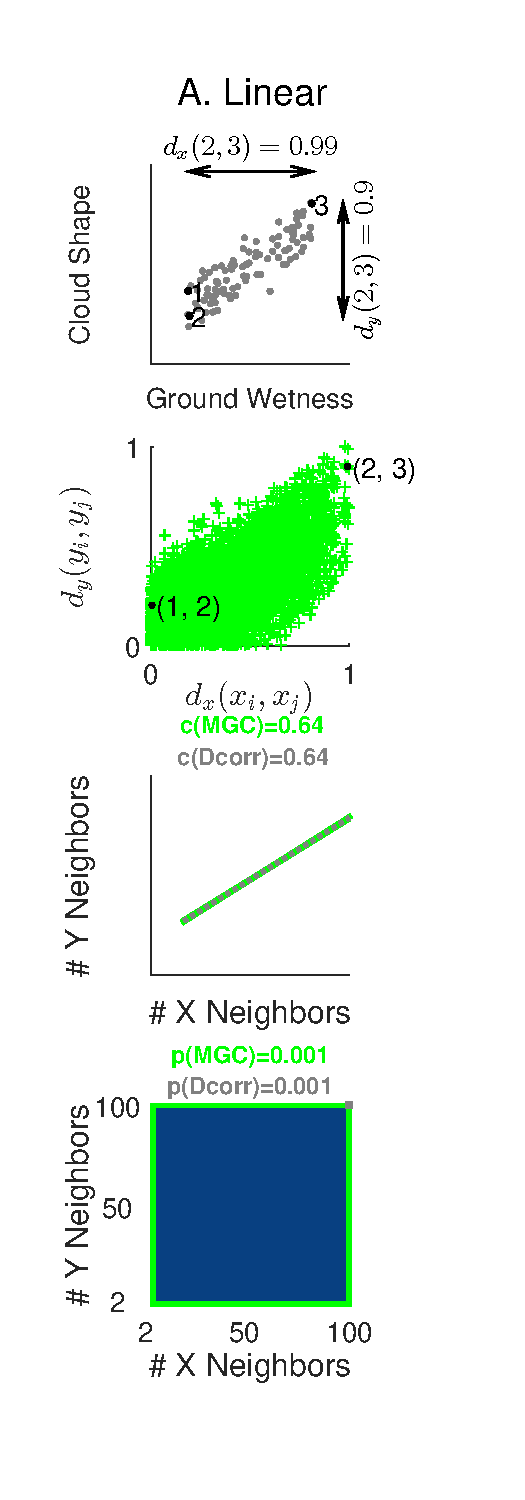
\includegraphics[width=1.0\textwidth]{Figures/Fig1}
\caption{
Powers of different methods for $20$ different $1$-dimensional simulations, estimated by the empirical distributions of the test statistics under the null and the alternative on the basis of $10$,$000$ Monte-Carlo replicates.
Each panel shows empirical testing power on the absicca, and sample size on the ordinate.
MGC empirically achieves similar or better power than the previous state of the art approaches for nearly all sample sizes on all problems.}
\label{fig:1D}
\end{figure}

For the $1$-dimensional simulations, MGC$\{$dcorr$\}$/$\{$mcorr$\}$/$\{$Mantel$\}$ either equals or is better than the corresponding global test in power. For dependencies that are close to linear (type 1-5), MGC always yields the same testing power as the global correlation, with HHG being slightly inferior; for the remaining nonlinear dependencies (type 6-19), HHG is the best among all benchmarks, yet MGC is able to achieve similar or better performance than HHG in almost all simulations. %although different MGC implementations vary slightly in the actual testing powers.

For all distributions other than the independent clouds, all empirical powers eventually increase to $1$ as the sample size increases, implying that all methods are consistent except the Mantel test, whose powers stay low in many nonlinear dependencies; and for the independent clouds, the empirical power of MGC is indeed around the type $1$ error level, so no false signal is detected once the optimal scale is determined. 

To better summarize the overall performance in the low-dimensional simulations, we use the performance profiles \cite{DolanMore2002}, which provides an intuitive way for directly comparing a set of algorithms on a set of problems.  Briefly, each curve (profile) shows the relative performance of a given algorithm as a function of how far from the best algorithm it performed. Therefore, higher curves and larger area under curve are better, and a more detailed description is in appendix section~\ref{appen:profiles}. For each $1$-dimensional simulation, we fix the sample size by a power threshold, and draw the corresponding performance profiles of all tests in figure~\ref{fig:pp}(A). To compare the performance profiles of each test with respect to different threshold choices, we further provide the area under curve of the performance profiles against the power threshold in figure~\ref{fig:pp}(B).
\begin{figure}
  \centering
  \begin{tabular}{@{}p{0.5\linewidth}@{\quad}p{0.5\linewidth}@{}}
    \subfigimg[width=\linewidth]{A}{Figures/Fig3} &
    \subfigimg[width=\linewidth]{B}{Figures/Fig4} \\
    \subfigimg[width=\linewidth]{C}{Figures/Fig7} &
    \subfigimg[width=\linewidth]{D}{Figures/Fig8}
  \end{tabular}
  \caption{Quantitative comparisons of the power of the various tests across all simulations into a single number.  
(A) Performance profile plots comparing different methods on all 1-dimensional simulations at the first sample size $n$ of any testing power to exceed the power threshold 0.8. The legend provides the Area-Under-the-Curve (AUC) for each method; larger is better.
(B) AUC for each method sweeping over all different power thresholds, the higher the better.
(C) Same as (A) but for the high-dimensional simulations, at the largest dimension of any testing power that is above the power threshold $0.5$.
(D) Same as (B) but for the high-dimensional simulations.
It is clear that MGC outperforms the previous state of the art approaches regardless of the underlying model, sample size, and dimensionality.}
\label{fig:pp}
\end{figure}

From figure~\ref{fig:pp}(A)(B), MGC is clearly more reliable than all benchmarks throughout the $1$-dimensional simulations regardless of the actual implementation. HHG is slightly better than dcorr / mcorr in the performance profiles, because there are more nonlinear simulations than linear in the $20$ dependencies, and HHG has a larger advantage for nonlinear dependency than its disadvantage in linear dependency; the global Mantel test has the lowest performance profile, but utilizing local correlations makes MGC$\{$Mantel$\}$ perform similarly as the other two MGC implementations.

\subsection{High-Dimensional Simulation Experiments}
\label{numer2}
In this section we consider the same $20$ distributions and the same testing procedures as in section~\ref{numer1}, but with increasing dimensions at a fixed sample size. For each dependency type, the testing powers are calculated against increasing $d_{x}$ with $d_{y}$ equals $d_{x}$ or $1$ depending on the particular distribution; and the sample size fixed at $n=100$.

The powers are shown in figure~\ref{fig:nD} against $d_{x}$, based on $r=10$,$000$ Monte-Carlo replicates at $\alpha=0.05$ (and $2$,$000$ additional MC replicates for optimal scale estimation). The performance profiles are provided in figure~\ref{fig:pp}(C)(D): figure~\ref{fig:pp}(C) draws the performance profiles of all methods at a fixed dimension determined by a power threshold; and figure~\ref{fig:pp}(D) plots the area under curve of the performance profiles against the power threshold.

Like the $1$-dimensional scenario, MGC either equals the corresponding global correlation (for type 1-5), or is significantly better (type 6-19) in testing powers due to its capability to better handle nonlinearity and high-dimensionality at the same time. In particular, MGC$\{$mcorr$\}$ enjoys a significant advantage over all benchmarks, since mcorr is more suitable for high-dimensional testing; and the performance profiles of MGC clearly reflect its overall superiority. 

In the following sections, unless mentioned otherwise, we concentrate on MGC$\{$mcorr$\}$, because the three different MGC implementations often yield similar numerical results with MGC$\{$mcorr$\}$ being more advantageous based on the high-dimensional simulations.

\begin{figure}[htbp]
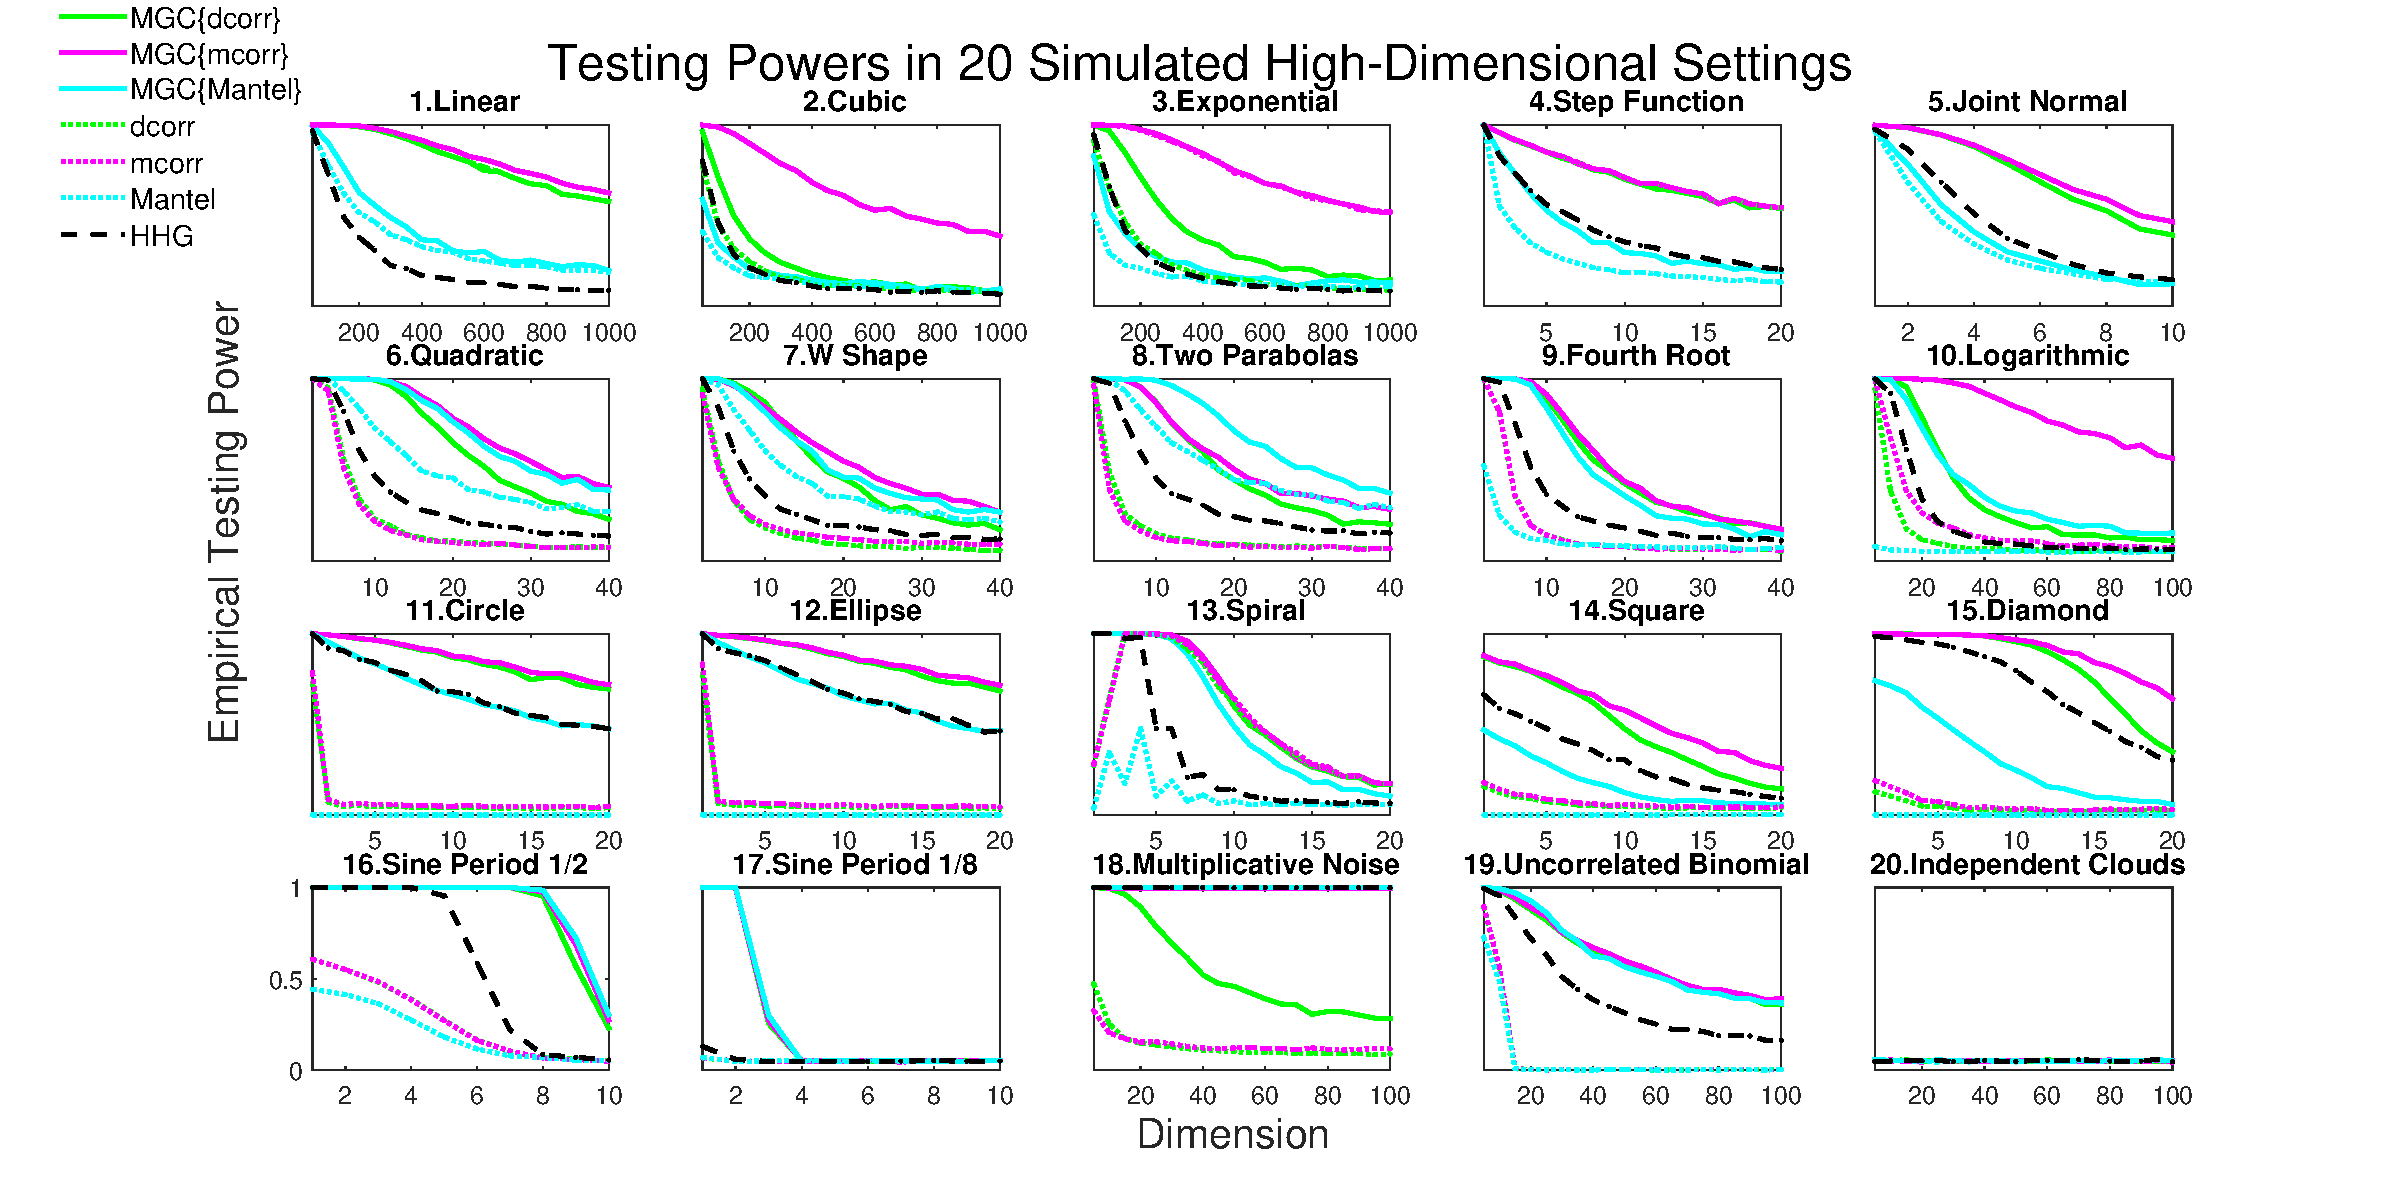
\includegraphics[width=1.0\textwidth]{Figures/Fig5}
\caption{Power of different methods on 20 different high-dimensional simulations, for dimensionality ranging from $1$ to $1$,$000$ at a fixed sample size $n=100$.  Details as in figure~\ref{fig:1D}.
Again, our method empirically achieves as high or higher power than the previous state of the art methods for nearly all problems and all dimensions.
}
\label{fig:nD}
\end{figure}

\subsection{Discovery of Dependency Across Scales}
\label{main3}

Figure~\ref{figSim6} illustrates how the powers of local correlations $\{\G_{kl}\}$ change with respect to increasing neighborhood $k$ and $l$, for the high-dimensional simulations (the $1$-dimensional case is included in appendix). They are plotted at a fixed sample size and a fixed dimension by the same power thresholds as in figure~\ref{fig:pp}(A)(C). 

The testing powers of all local correlations also shed light into the intrinsic dependency structure: for dependencies that are close to linear (type 1-5), the best neighborhood choice is always the largest scale, i.e., $k=l=n$; but for all other nonlinear dependencies (type 6-19), MGC almost always chooses a smaller scale, which is distribution dependent. Furthermore, similar dependencies have similar local correlation structure, and thus similar optimal scales. For example, type 6 and type 7 are both polynomials of degree 2 with different coefficients, so the optimal scales are quite similar to each other; type 16 and 17 are the same trigonometry function with different periods, and they share a narrow range of significant local correlations; so are circle and eclipse, square and diamond, etc. Note that for almost all simulations, there exist a large portion of adjacent local correlations that are equally significant, which is an important observation that we use to approximate the MGC optimal scale for one pair of data with unknown model in appendix section~\ref{appen:tests}.

\begin{figure}[htbp]
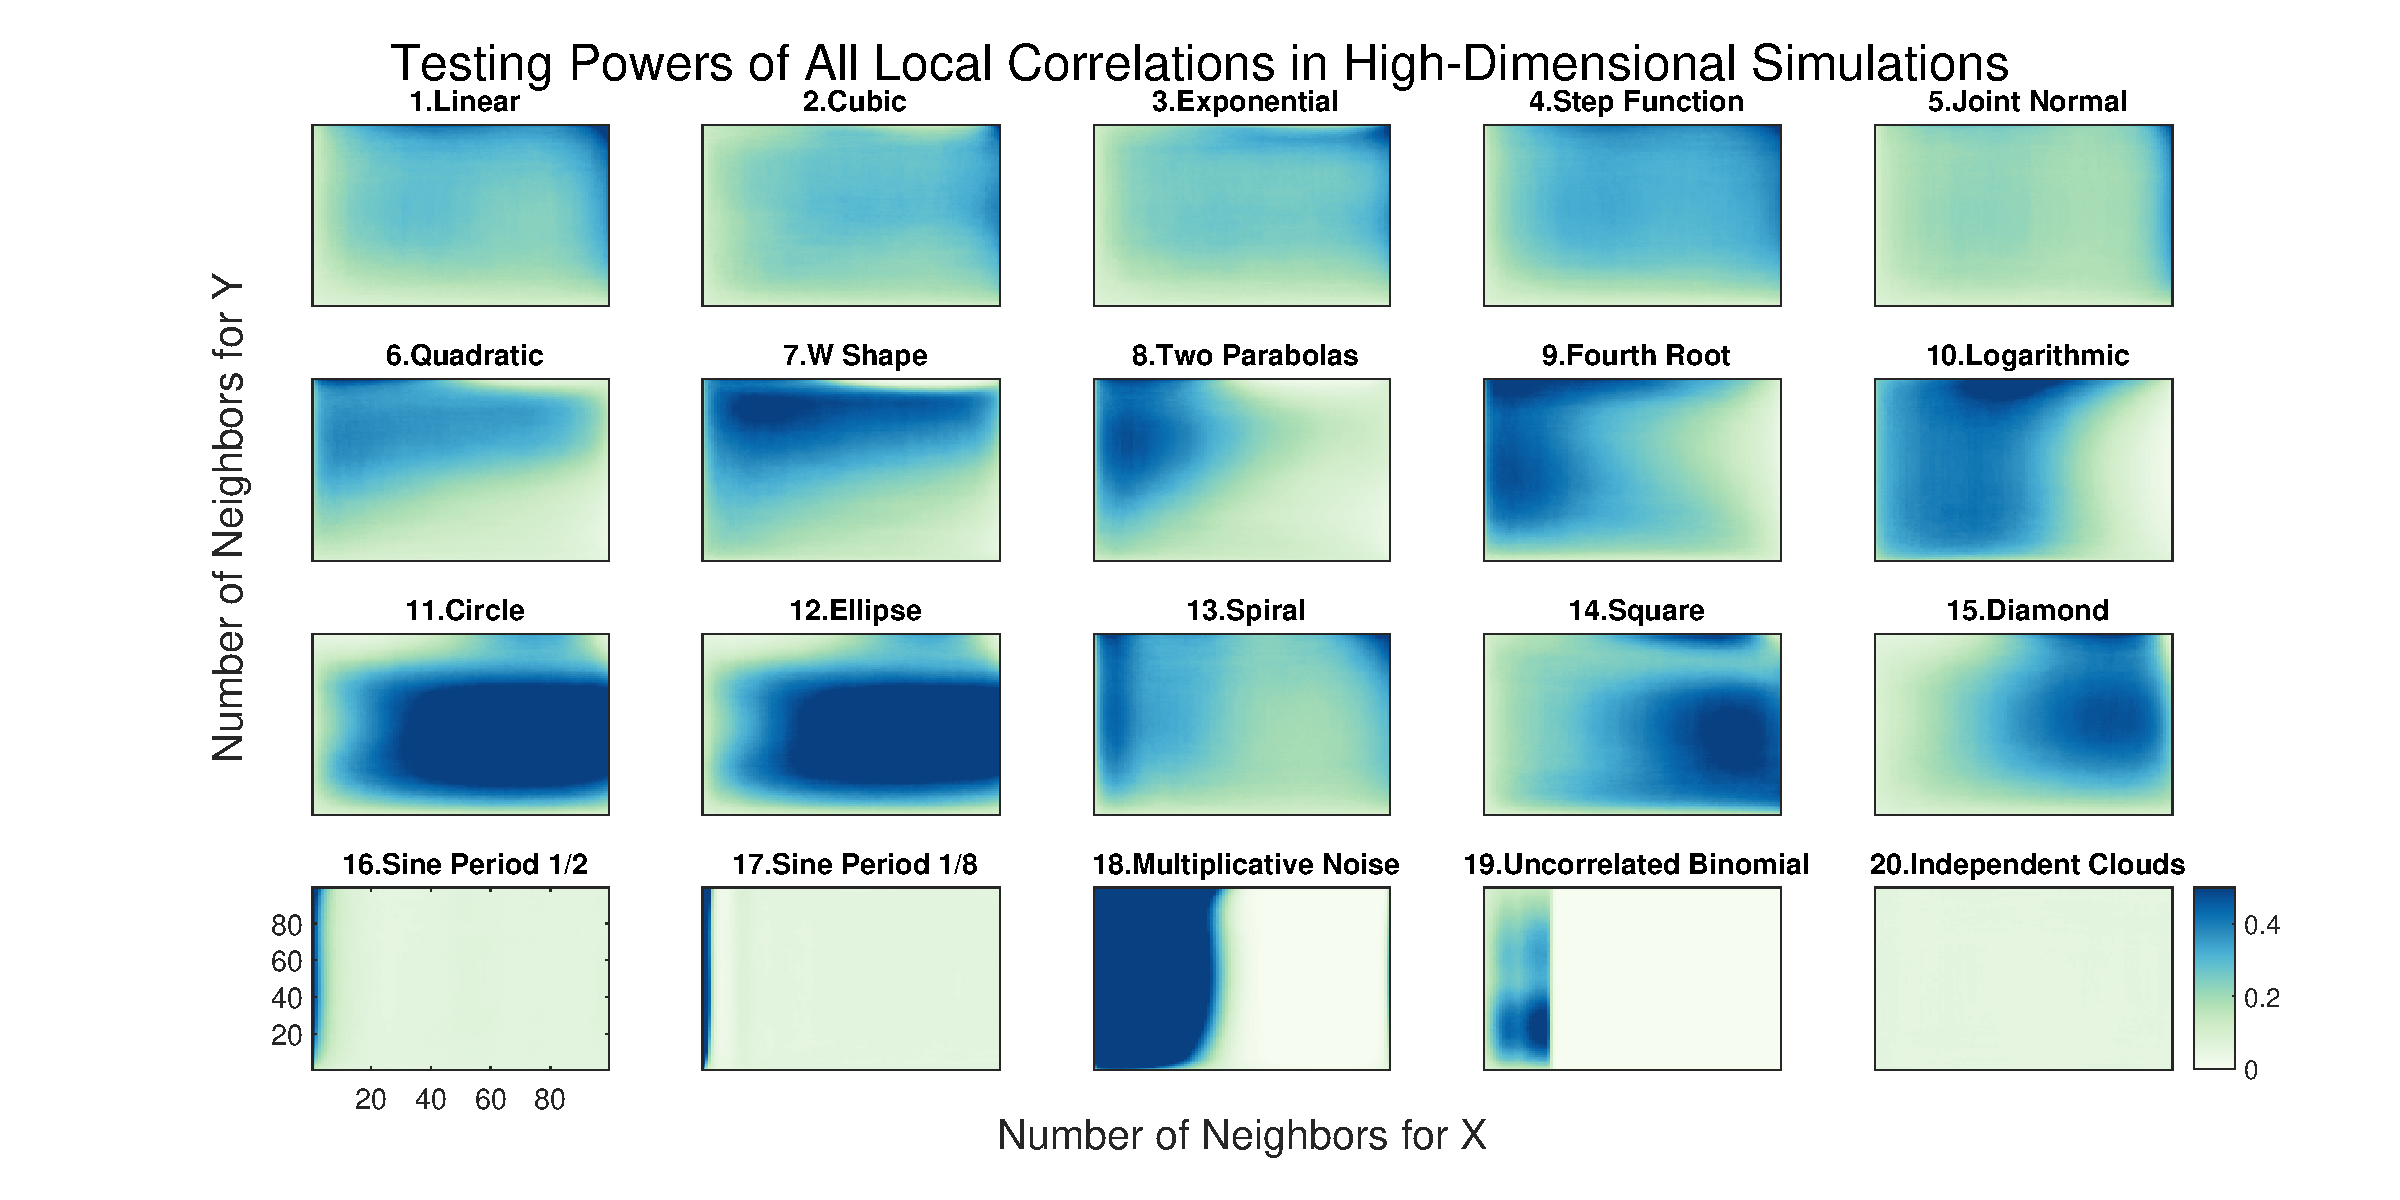
\includegraphics[width=1.0\textwidth]{Figures/Fig6}
\caption{Testing power heat map of local mcorr correlations with respect to number of neighbors for high-dimensional simulations.
For each of the 20 panels, the abscissa denotes the number of neighbors for $X$ (the scale increases from left to right), and the ordinate denotes the number of neighbors for $Y$ (the scale increases from bottom to top). For each simulation, the sample size is $n=100$, and the dimension is determined by the power threshold as in figure~\ref{fig:pp}(C). Each different simulation yields a different surface, highlighting the importance of understanding local scale in terms of understanding the data. }
\label{figSim6}
\end{figure}

To characterize the above behaviors, in the following theorems we prove that: for the testing power of the permutation test, MGC indeed equals the global correlation under linear dependency, i.e., the largest scale $(n,n)$ is an optimal scale for MGC; but under certain nonlinear dependency, MGC may enjoy a better finite-sample testing power than the corresponding global correlation. 

\begin{thm}
\label{thm2}
Suppose $\mb{x}$ is linearly dependent of $\mb{y}$. Then for any $n$ and $\alpha$ it always holds that
\begin{equation}
\beta_{\alpha}(\G^{*}) = \beta_{\alpha}(\G).
\end{equation}

Thus multiscale graph correlation is equivalent to the global correlation coefficient under linear dependency.
\end{thm}

\begin{thm}
\label{thm3}
There exists $f_{xy}$, $n$ and $\alpha$ such that 
\begin{equation}
\beta_{\alpha}(\G^{*}) > \beta_{\alpha}(\G).
\end{equation}

Thus multiscale graph correlation can be better than its global correlation coefficient under certain nonlinear dependency.
\end{thm}
Note that Theorem~\ref{thm2} and Theorem~\ref{thm3} hold for MGC implemented by any of dcorr / mcorr / Mantel.

The proof of Theorem~\ref{thm3} is a constructive one, as it shows that local correlation can outperform its global counterpart even for the most modest nonlinear functions, such as a quadratic.  Because any function can be approximated by a polynomial expansion \cite{RudinBook}, the proof of Theorem~\ref{thm3} suggests that MGC is able to outperform the corresponding global correlation on a wide variety of nonlinear functions, which is indeed the case throughout the numerical simulations.


\subsection{Robustness against Outliers}
\label{main4}
To show that MGC is robust against ourliers, let us consider a simple mixture model: suppose the joint distribution satisfies $f_{xy}=p f_{1}+(1-p) f_{2}$, where $f_{1} \sim \mc{N}(\mu_{1},\Sigma_{1})$ and $f_{2} \sim \mc{N}(\mu_{2},\Sigma_{2})$. We set $\mu_{1}=(0,0)$, $\mu_{2}=(5,-5)$, $\Sigma_{1} = \begin{bmatrix} 1&1\\ 1&1 \end{bmatrix}$, and $\Sigma_{2} = \begin{bmatrix} 1&0\\ 0&1 \end{bmatrix}$. Namely $x=y$ with probability $p$, otherwise independently normally distributed. Given $p$, the simulating sample pairs $(X,Y)$ at $n=100$ can be repeatedly generated to estimate the testing powers at $\alpha=0.05$. 

For sample data generated from the mixture model, there are around $pn$ observations in $X$ that are exactly the same as the corresponding observations in $Y$; and the remaining observations in $X$ are outliers, which are independent of the corresponding observations in $Y$. One such sample pair $(X,Y)$ at $p=0.5$ and $n=100$ is plotted in figure~\ref{figSim3}(A), and the testing powers of all local mcorr correlations are shown in figure~\ref{figSim3}(B)(C)(D) for $p=0.3$,$0.5$,$0.7$ respectively, using the same procedure as in section~\ref{numer1}.

The optimal local mcorr is clearly much better than global mcorr. Furthermore, the optimal scale $(k^{*},l^{*})$ is directly related to the mixture probability $p$, where $k^{*}=l^{*}=\min(pn,(1-p)n)-1$ is always optimal. Intuitively, MGC is robust against outliers as the optimal local correlation automatically excludes the independent outliers from the dependent observations in testing. The robustness still holds as the dimension, sample size, or the underlying dependency change, which makes MGC more advantageous in practice against noise and outliers. 

\begin{figure}
  \centering
  \begin{tabular}{@{}p{0.5\linewidth}@{\quad}p{0.5\linewidth}@{}}
    \subfigimg[width=\linewidth]{A}{Figures/FigOut0} &
    \subfigimg[width=\linewidth]{B}{Figures/FigOut1} \\
    \subfigimg[width=\linewidth]{C}{Figures/FigOut2} &
    \subfigimg[width=\linewidth]{D}{Figures/FigOut3}
  \end{tabular}
  \caption{Testing power heat map of local mcorr correlations with respect to number of neighbors for the mixture model.
(A) Scatter plot of sample $(X,Y)$ under the mixture model with probability $p=0.5$
(B) Testing power of all local correlation under the mixture model with probability $p=0.3$.
(C) Same as (B) with $p=0.5$.
(D) Same as (B) with $p=0.7$.
MGC is always better than global mcorr, and the local powers imply the existence of outliers.}
\label{figSim3}
\end{figure}

\subsection{Real Data Experiments}

\label{numer3}
Here we apply local correlations and MGC to visualize the relationship and test independence between real data sets. Since there is no known model for the given data, the optimal scale for MGC is approximated based on the p-values of all local correlations from the permutation test (see appendix section~\ref{appen:tests} for details and further discussions). 

\subsubsection{Local Scales can Detect Dependence Between Hippocampus Shape and Depression}

The first experiment is to test dependency between the brain hippocampus shape and major depressive disorder. There are $n=114$ subjects, and the brain images of each person are obtained by high resolution MRI scans on the hippocampus for both the left brain and the right brain. A categorical vector containing the disorder information is also available, including clinically depressed subject, high-risk subject, and non-affected subject. There has been evidences that relate major depressive disorder to the hippocampus shape in \cite{ParkEtAl2011} and \cite{PosenerEtAl2003}, and we would like to test the significance of such relationship in the raw data. 

To start with, we transform the respective data sets into dissimilarity matrices: for the brain data, two dissimilarity matrices representing the left and right hippocampus data are obtained based on landmark matching (see \cite{ParkEtAl2011} for more details on data processing); for the disorder information vector,
we form the pairwise Euclidean distance matrix from the categorical vector, then add $1$ to every non-diagonal entry (so only the diagonals are of distance $0$).

Two hypothesis tests are considered: testing dependency between the left brain and major depressive disorder, and testing dependency between the right brain and major depressive disorder. The resulting p-values based on $r=10$,$000$ random permutations are reported in the first two rows of Table~\ref{table1}. For testing between the left brain and the disorder, MGC / HHG / Mantel yield significant p-values with dcorr / mcorr being slightly higher than significance; for testing between the right brain and the disorder, only MGC yields significant p-value, and all benchmarks have p-values higher than significance. 

The p-value curves of the local correlations are provided in figure~\ref{figReal}(A) for $k=2,\ldots,n$ at $l=4$, since the largest rank is $4$ for the categorical vector. We can clearly identify many common local scales between the two curves that yield significant p-values, which is the reason that MGC can successfully identify the signals in both tests, and implies a similar local dependency structure. 

\begin{table*}[!t]
\Large
\renewcommand{\arraystretch}{0.5}
\centering
{\begin{tabular}{|c||c|c|c|c|c|c|c|}
\hline
Testing Method & MGC & dcorr & mcorr & Mantel & HHG \\
\hline
Left Brain vs Disorder  & $\textbf{0.0046}$ & $0.0745$ & $0.0783$ & $0.0382$ & $0.0375$ \\
\hline
Right Brain vs Disorder & $\textbf{0.0133}$ & $0.1046$ & $0.1104$  & $0.0848$ & $0.0809$\\
\hline
\Migraine~vs CCI & $0.0111$ & $\textbf{0.0088}$ & $0.0111$  & $0.0093$ & $0.0341$\\
\hline
\mtg~vs CCI & $0.0712$ & $\textbf{0.0682}$ & $0.0712$  & $0.3314$ & $0.6553$\\
\hline
\end{tabular}
\caption{The p-values by the permutation test, for testing dependence on $4$ different pairs of real data. MGC is able to consistently identify significant relationship for the first three rows, and does not inflate the p-value in the last row.}
\label{table1}
}
\end{table*}

\begin{figure}
  \centering
  \begin{tabular}{@{}p{0.5\linewidth}@{\quad}p{0.5\linewidth}@{}}
    \subfigimg[width=\linewidth]{A}{Figures/FigReal1} &
    \subfigimg[width=\linewidth]{B}{Figures/FigReal2} \\
    \subfigimg[width=\linewidth]{C}{Figures/FigReal3} &
    \subfigimg[width=\linewidth]{D}{Figures/FigReal4}
  \end{tabular}
\caption{
(A) Local correlation p-value curves with respect to $k=2,\ldots,114$ at $l=4$ for brain vs disease. 
(B) False positive rates for brain vs noise throughout $26$ different data sets. 
(C) Local correlation p-value heat map with respect to $k=2,\ldots,109$ and $l=2,\ldots,38$ for brain \Migraine~vs CCI.
(D) Local correlation p-value heat map with respect to $k=2,\ldots,109$ and $l=2,\ldots,38$ for brain \mtg~vs CCI. }
\label{figReal}
\end{figure}

\subsubsection{MGC can Select Amongst Disparate Representations for Optimal Dependence: Brain Structural Network vs. Creativity}

Next we experiment on \Migraine~vs CCI and \mtg~vs CCI. More specifically, we estimated brain graphs from diffusion MRI data using two different pipelines, one called \Migraine, and the other called \mtg.  The question we have is whether brain graphs are independent of creativity.  Because we cannot directly measure brain graphs, we must estimate them from the data.  Currently, the jury is out on which estimation procedure is best.  Therefore, we tried both to determine which worked better for this particular task.

Using the same testing procedure as the previous experiment, the resulting p-values for \Migraine~vs CCI and \mtg~vs CCI are reported in the last two rows of Table~\ref{table1}. The dependency between \Migraine~and CCI is strong enough for all methods to return significant p-values. But there appears to be a loss of dependency between \mtg~and CCI, as neither the global methods nor MGC return significant p-values. 

From the local correlation p-value heat maps in figure~\ref{figReal}(C)(D), we observe that there exists many local scales with significant p-values for \Migraine~vs CCI, which is no longer the case for \mtg~vs CCI. In comparison, global methods do not exhibit the local structure; and Mantel and HHG are less informative due to the large change of p-values when moving from \Migraine~to \mtg. Note that if we test independence between \Migraine~vs \mtg, the p-values of all tests are $0$, indicating a strong dependency. 

Therefore in this exploration task, \Migraine~is a better brain graph estimator than \mtg: although they are strongly related with each other, \Migraine~is more dependent with CCI than \mtg, because \mtg~is a transformation of \Migraine~without consideration of CCI. Our method identifies the better representation of the two, reveals the local dependency loss from the p-value heat maps, and does not identify false signals. Thus MGC can be used to find the most relevant representation / variable and provide valuable insights into the structural difference.

\subsubsection{MGC Does Not Inflate False Positive Rates: Brain Activity vs. Noise}

In the last experiment, MGC is applied to test independence between brain voxel activities and non-existent stimulus similar to \cite{EklundKnutsson2012}, by using $26$ resting state fMRI data sets from the Neuroimaging Informatics Tools and Resources Clearinghouse (NITRC) 1000 functional connectomes project \url{http://fcon_1000.projects.nitrc.org/}. Take one data set BNU1 for example: the resting state data contains $200$ regions of interest for $200$ timestep for $50$ persons; and there are two resting state data for the same person. We used CPAC to estimate regional time-series, in particular, using the sequence of pre-processing decisions determined to optimize discriminability (unpublished).

For each brain region, the distance matrix with respect to time is calculated by $dist(s,t)=\|x_{\cdot s}-x_{\cdot t}\|$, where $x_{\cdot t}$ denote the observation vector at timestep $t$ for all persons. Then an independent stimulus is generated by sampling from a standard normal at each time step, whose pairwise distance can be directly computed. From the two distance matrices, we test the dependency between each brain region and the time-varying stimulus by MGC. The p-value based on $1000$ random permutations is computed, and each brain region is declared significant when the p-value is less than $\alpha=0.05$. Note that the distance matrices at different brain regions are distinct, but the stimulus is the same for all brain regions during the same experiment.

For each data set, the above testing is carried out for each brain region, and the false positive rate (FDR) of MGC is shown in figure~\ref{figReal}(B). The y-axis stands for FDR by log scale, and the x-axis shows the name of the data set arranged by increasing FDR; the mean FDR of MGC is shown as the purple-red straight line, with the type $1$ error level $0.05$ drawn as the blue straight line. As the stimulus is in fact independent of the brain activities, the false positive rate should be close to $\alpha=0.05$ for each data set. This is indeed the case for MGC, and the actual mean/standard deviation is $0.060 \pm 0.025$. This is in contrast to many other methods that may significantly increase FDR as reported in \cite{EklundKnutsson2012} for the same data source.

\section{Discussion}
\label{conclu}

\paragraph{Summary}
In short, we propose multiscale graph correlation to test independence between data sets, which has been shown to be perform well for testing independence on data of small sample size, low- or high-dimensionality, linearity or nonlinearity, etc. It not only enjoys theoretical guarantee such as being consistent in testing independence, but also exhibits superior numerical performances in a comprehensive simulation setting and real data experiments, comparing to existing popular methods. Therefore, the concept of local correlation coefficient and MGC shall find many good applications in various domains that involve discovering relationship among multiple data. 

\paragraph{Next Steps}
Although our definition of local correlation coefficient is fast to implement, generally applicable to any global correlation, and achieves good testing powers, there are multiple ways to combine neighborhood information into a particular global correlation coefficient. So it is possible that the testing performance may be further improved by tailoring a different centering or ranking scheme for a given global correlation, which is a worthwhile direction for future works. Furthermore, future investigations on the optimal scale for MGC is also of interest, such as how to more accurately select the local scale under unknown models for a particular inference task, and the implication of the optimal scale on the geometry of underlying dependency, etc. Beyond the testing framework, it may also be promising to pursue the applications of MGC and local correlations in other closely-related subjects like dimension reduction and supervised learning. 

%scaling up via FlashX?

\section*{Acknowledgment}
\addcontentsline{toc}{section}{Acknowledgment}
This work was partially supported by 
% 
National Security Science and Engineering Faculty Fellowship (NSSEFF), 
% 
Johns Hopkins University Human Language Technology Center of Excellence (JHU HLT COE), 
% 
Defense Advanced Research Projects Agency's (DARPA) SIMPLEX program through SPAWAR contract N66001-15-C-4041, 
% 
and the XDATA program of the Defense Advanced Research Projects Agency (DARPA) administered through Air Force Research Laboratory contract FA8750-12-2-0303.



\appendix
\setcounter{figure}{0}
\renewcommand\thefigure{A\arabic{figure}} 

\section{Simulation Functions}
\label{appen:function}

We list the distributions of the $20$ dependencies used in the simulations, which are based on a combination of the simulations used in \cite{SzekelyRizzoBakirov2007, SimonTibshirani2012, SimonTibshirani2012, GorfineHellerHeller2012} but with some changes (such as the inclusion of additional noise and an extra weight vector) to better compare all methods in our low- and high-dimensional simulations.

For each sample $x \in \Real^{d_{x}}$, we denote $x^{d}, d=1,\ldots,d_{x}$ as the $d$th dimension of $x$. For the purpose of high-dimensional simulations, $w \in \Real^{d_{x}}$ is a decaying vector with $w^{d}=1/d$ for each $d$, such that $w\T x$ is a $1$-dimensional weighted summation of all dimensions of $x$, which equals $x$ if $d_{x}=1$. Furthermore, $\mc{U}$ denotes the uniform distribution, $\mc{B}$ denotes the Bernoulli distribution, $\mc{N}$ denotes the normal distribution, $u$ and $v$ represent realizations from some auxiliary random variables, $c$ is a scalar constant to control the noise level (which equals $1$ for 1-dimensional simulations and $0$ otherwise), and $\epsilon$ is sampled from an independent standard normal distribution unless mentioned otherwise. 

For all of the below equations, $(x,y) \overset{iid}{\sim} f_{xy} = f_{y|x} f_x$. For each setting, we provide the space of $(x,y)$, and define each of the above distributions, and any additional auxiliary distributions.

\setcounter{equation}{0}
\begin{compactenum}
\item Linear $(x,y) \in \Real^{d_{x}} \times \Real$,  
\begin{align*}
x &\sim \mc{U}(-1,1)^{d_{x}},\\
y &=w\T x+c\epsilon.
\end{align*}
\item Cubic $(x,y) \in \Real^{d_{x}} \times \Real$: 
\begin{align*}
x &\sim \mc{U}(-1,1)^{d_{x}}, \\ 
y &=128(w\T x-\tfrac{1}{3})^3+48(w\T x-\tfrac{1}{3})^2-12(w\T x-\tfrac{1}{3})+80c\epsilon.
\end{align*}
\item Exponential $(x,y) \in \Real^{d_{x}} \times \Real$: 
\begin{align*}
x &\sim \mc{U}(0,3)^{d_{x}}, \\
y &=exp(w\T x)+10c\epsilon.
\end{align*}
\item Step Function $(x,y) \in \Real^{d_{x}} \times \Real$: 
\begin{align*}
x &\sim \mc{U}(-1,1)^{d_{x}},\\ 
y &=\mb{I}(w\T x>0)+\epsilon,
\end{align*}
where $\mb{I}$ is the indicator function. 
\item Joint normal $(x,y) \in \Real^{d_{x}} \times \Real^{d_{x}}$: Let $\rho=1/2d_{x}$, $I_{d_{x}}$ be the identity matrix of size $d_{x} \times d_{x}$, $J_{d_{x}}$ be the matrix of ones of size $d_{x} \times d_{x}$, and $\Sigma = \begin{bmatrix} I_{d_{x}}&\rho J_{d_{x}}\\ \rho J_{d_{x}}&I_{d_{x}} \end{bmatrix}$. Then let $(u,v) \sim \mc{N}(0, \Sigma)$, $\epsilon \sim \mc{N}(0, I_{d_{x}})$,
\begin{align*}
x &=u,\\ 
y &=v+0.5c\epsilon.
\end{align*}
\item Quadratic $(x,y) \in \Real^{d_{x}} \times \Real$: 
\begin{align*}
x &\sim \mc{U}(-1,1)^{d_{x}},\\
y&=(w\T x)^2+0.5c\epsilon.
\end{align*}
\item W Shape $(x,y) \in \Real^{d_{x}} \times \Real$:  $u \sim \mc{U}(-1,1)^{d_{x}}$,
\begin{align*}
x &\sim \mc{U}(-1,1)^{d_{x}},\\
y&=4\left[ \left( (w\T x)^2 - \tfrac{1}{2} \right)^2 + w\T u/500 \right]+0.5c\epsilon.
\end{align*}
\item Two Parabolas $(x,y) \in \Real^{d_{x}} \times \Real$: $\epsilon \sim \mc{U}(0,1)$, $u \sim \mc{B}(0.5)$,
\begin{align*}
x &\sim \mc{U}(-1,1)^{d_{x}},\\
y&=\left( (w\T x)^2  + 2c\epsilon\right) \cdot (u-\tfrac{1}{2}).
\end{align*}
\item Fourth Root $(x,y) \in \Real^{d_{x}} \times \Real$: 
\begin{align*}
x &\sim \mc{U}(-1,1)^{d_{x}},\\
y&=|w\T x|^\frac{1}{4}+\frac{c}{4}\epsilon.
\end{align*}
\item Logarithmic $(x,y) \in \Real^{d_{x}} \times \Real^{d_{x}}$: $\epsilon \sim \mc{N}(0, I_{d_{x}})$
\begin{align*}
x &\sim \mc{N}(0, I_{d_{x}}),\\
y^{d}&=2log(x^{d})+3c\epsilon^{d},
\end{align*}
for $d=1,\ldots,d_{x}$.
\item Circle $(x,y) \in \Real^{d_{x}} \times \Real$: $u \sim \mc{U}(-1,1)^{d_{x}}$, $\epsilon \sim \mc{N}(0, I_{d_{x}})$, $r=1$,
\begin{align*}
x^{d}&=r \left(\sin(\pi u^{d+1})  \prod_{j=1}^{d} \cos(\pi u^{j})+0.4 \epsilon^{d}\right) \mbox{ for $d=1,\ldots,d_{x}-1$},\\
x^{d_{x}}&=r \left(\prod_{j=1}^{d_{x}} \cos(\pi u^{j})+0.4 \epsilon^{d_{x}}\right),\\
y&= \sin(\pi u^{1}).
\end{align*}
\item Ellipse $(x,y) \in \Real^{d_{x}} \times \Real$: Same as above except $r=5$.

\item Spiral $(x,y) \in \Real^{d_{x}} \times \Real$: $u \sim \mc{U}(0,5)$, $\epsilon \sim \mc{N}(0, 1)$, 
\begin{align*}
x^{d}&=u \sin(\pi u)  [\cos(\pi u)]^{d} \mbox{ for $d=1,\ldots,d_{x}-1$},\\
x^{d_{x}}&=u [\cos(\pi u)]^{d_{x}},\\
y&= u \sin(\pi u) +0.4 (d_{x}-1)\epsilon.
\end{align*}

\item Square $(x,y) \in \Real^{d_{x}} \times \Real^{d_{x}}$: Let $u \sim \mc{U}(-1,1)$, $v \sim \mc{U}(-1,1)$, $\epsilon \sim \mc{N}(0,1)^{d_{x}}$, $\theta=-\frac{\pi}{8}$. Then
\begin{align*}
x^{d}&=u \cos\theta + v \sin\theta + 0.05 d_{x}\epsilon^{d},\\
y^{d}&=-u \sin\theta + v \cos\theta,
\end{align*}
for $d=1,\ldots,d_{x}$.
\item Diamond $(x,y) \in \Real^{d_{x}} \times \Real^{d_{x}}$: Same as above except $\theta=-\frac{\pi}{4}$.
\item Sine Period 1/2 $(x,y) \in \Real^{d_{x}} \times \Real$: $u \sim \mc{U}(-1,1)$, $v \sim \mc{N}(0,1)^{d_{x}}$, $\theta=4\pi$,
\begin{align*}
x^{d}&=u+0.02 d_{x} v^{d} \mbox{ for $d=1,\ldots,d_{x}$}, \\
y&=\sin ( \theta x )+c\epsilon.
\end{align*}
\item Sine Period 1/8 $(x,y) \in \Real^{d_{x}} \times \Real$: Same as above except $\theta=16\pi$ and the noise is changed to $0.5c\epsilon$.
\item Multiplicative Noise $(x,y) \in \Real^{d_{x}} \times \Real^{d_{x}}$: $u \sim \mc{N}(0, I_{d_{x}})$, $\epsilon \sim \mc{N}(0, I_{d_{x}})$,
\begin{align*}
x &\sim \mc{N}(0, I_{d_{x}}),\\
y^{d}&=u^{d}x^{d}+0.5c\epsilon^{d},
\end{align*}
for $d=1,\ldots,d_{x}$.
\item Uncorrelated Binomial $(x,y) \in \Real^{d_{x}} \times \Real$: $u \sim \mc{B}(0.5)$,
\begin{align*}
x &\sim \mc{B}(0.5)^{d_{x}},\\ 
y&=(2u-1)w\T x+0.6\epsilon.
\end{align*}
\item Independent Clouds $(x,y) \in \Real^{d_{x}} \times \Real^{d_{x}}$: Let $u \sim \mc{N}(0,I_{d_{x}})$, $v \sim \mc{N}(0,I_{d_{x}})$, $u' \sim \mc{B}(0.5)^{d_{x}}$, $v' \sim \mc{B}(0.5)^{d_{x}}$. Then
\begin{align*}
x&=u/3+2u'-1,\\
y&=v/3+2v'-1.
\end{align*}
\end{compactenum}

For each distribution, $\mb{x}$ and $\mb{y}$ are clearly dependent except type 20; for some types (type 11-15) they are conditionally independent upon conditioning on the respective auxiliary variables, while for others they are "directly" dependent. Then we can independently generate $(x_{i},y_{i})$ from $(\mb{x},\mb{y})$ for $i=1,\ldots,n$, set $X=[x_{1},\cdots, x_{n}] \in \Real^{d_{x} \times n}$ and $Y=[y_{1},\cdots, y_{n}] \in \Real^{d_{y} \times n}$, and calculate local / global correlations for the sample data.

The low-dimensional simulations always set $d_{x}=d_{y}=1$ and $c=1$, with their visualizations shown in figure~\ref{fig0}. The parameter before $c$ (e.g., there is a $80$ before $c$ in type 2) is a tuned noise parameter for some dependencies, so the testing powers can be compared meaningfully for each simulation, e.g., in the absence of noise, the testing powers may converge to $1$ at very small $n$ for some trivial dependencies like linear; and it is also more meaningful to consider noisy simulations in practice. 

The high-dimensional simulations always set $c=0$ and $n=100$, with $d_{y}$ increasing while $d_{y}=d_{x}$ for type $5,10,14,15,18,20$ and $1$ otherwise. The decaying vector $w$ is utilized in most high-dimensional simulations, which treats higher dimensions as small perturbations and thus creates meaningful settings for testing power comparison. %but for some complex dependencies like square / diamond / sine period, the testing is already very difficult at $d_{x}>1$ and $w$ is not used.

\begin{figure}[htbp]
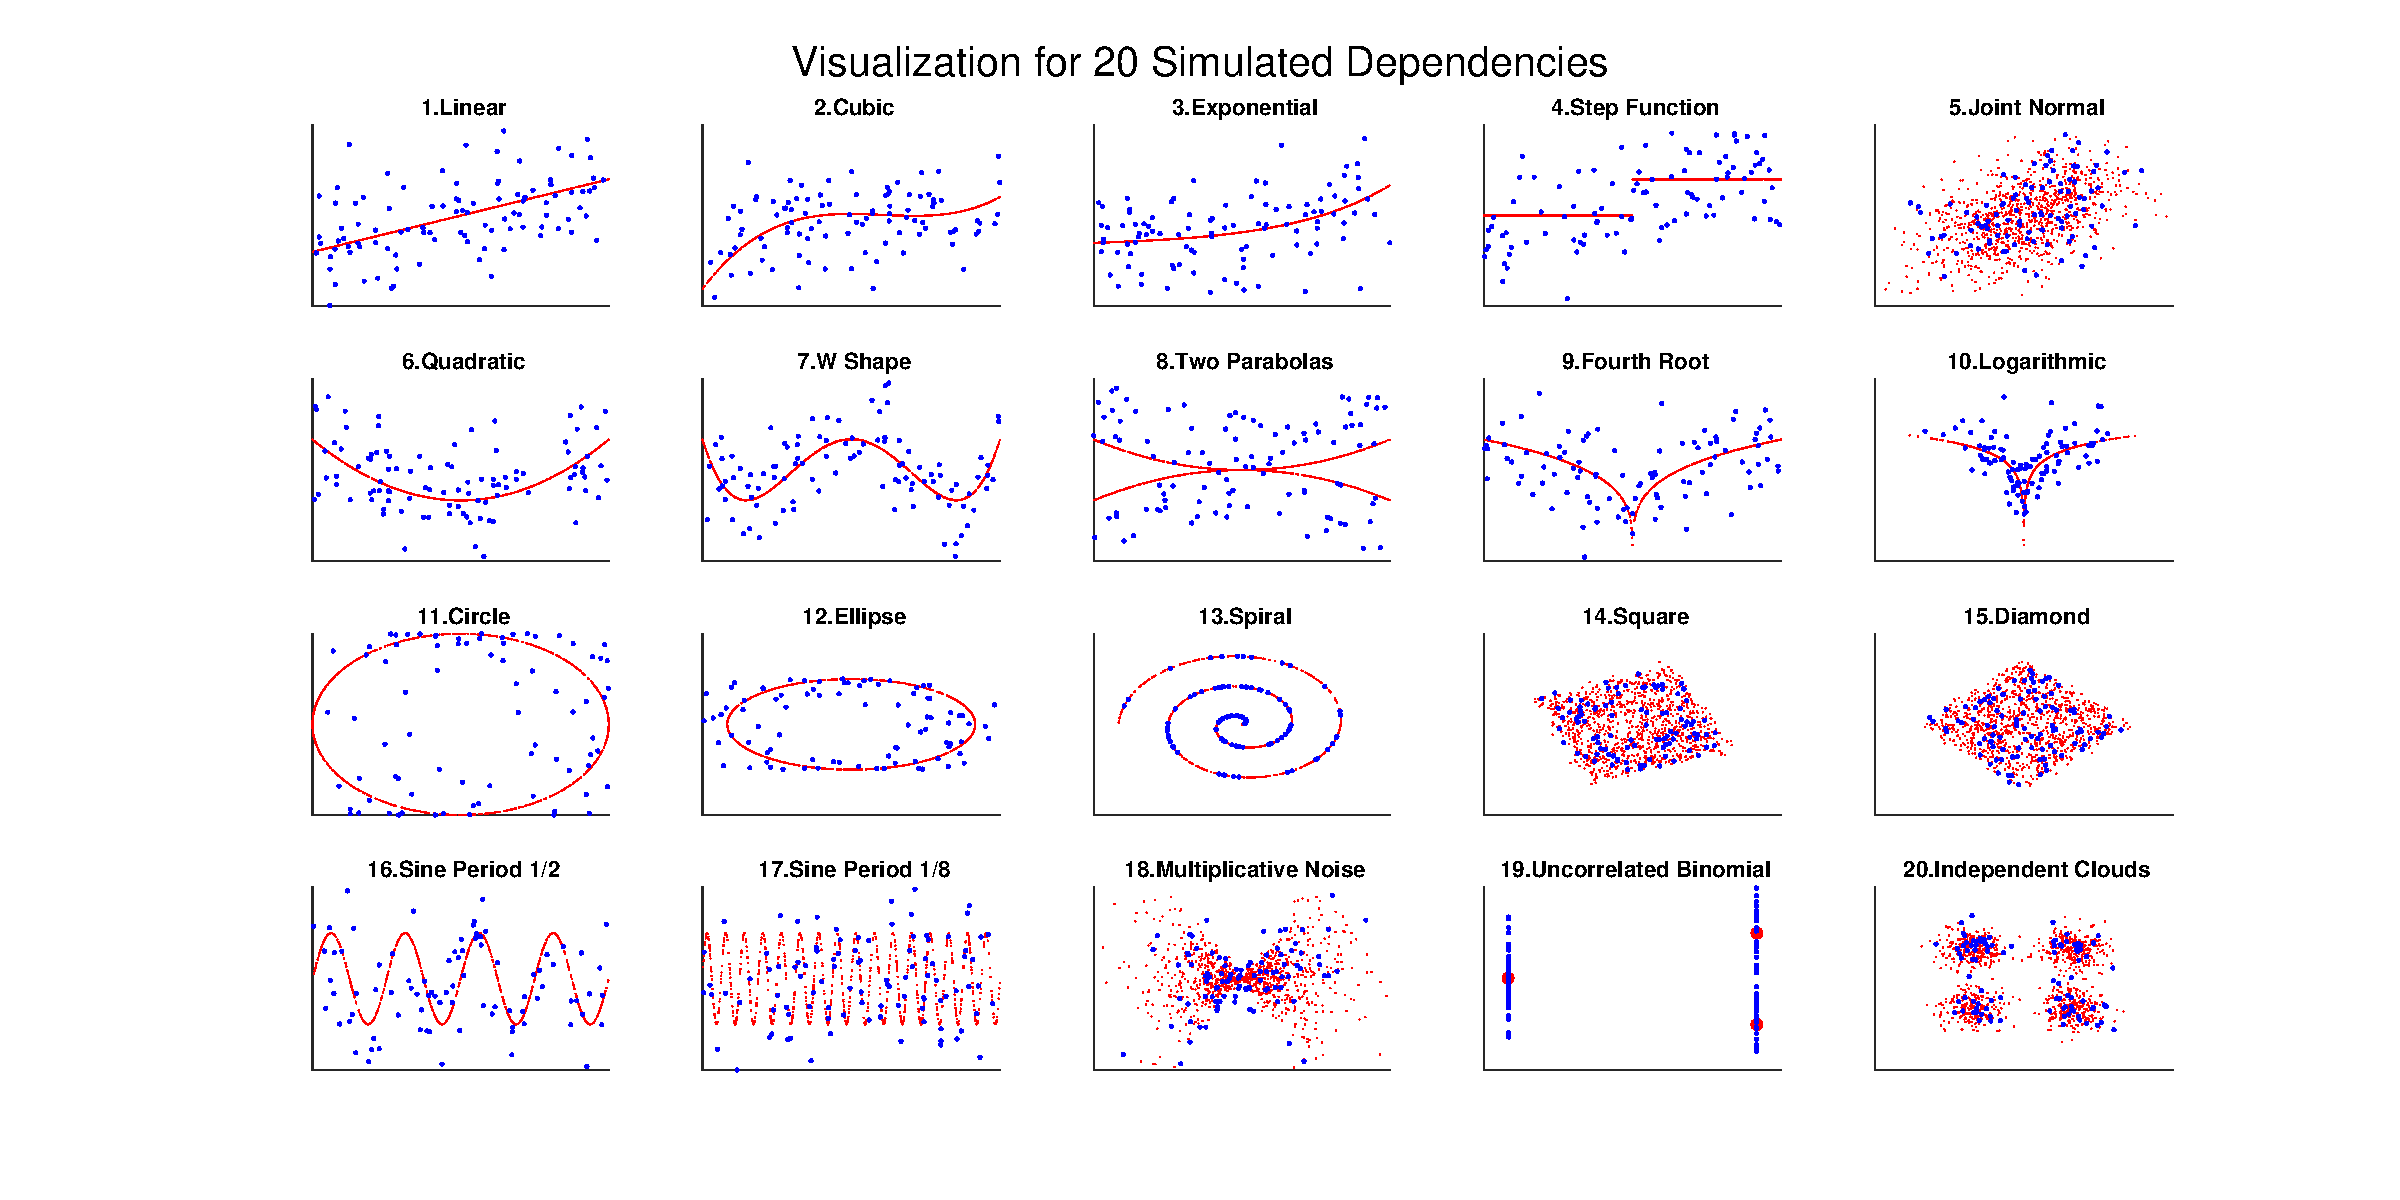
\includegraphics[trim={5cm 0 3.5cm 0},clip, width=1.0\textwidth]{Figures/Fig0}
\caption{Visualization of the $20$ dependencies for $1$-dimensional simulations. The blue points are generated with noise (c=1) at $n=100$ to show the actual sample data in testing, and the red points are generated without noise at $n=1000$ to highlight each underlying dependency.
}
\label{fig0}
\end{figure}

The testing power heat map of local correlations for the $1$-dimensional simulations is provided in figure~\ref{figSim2}.
\begin{figure}[htbp]
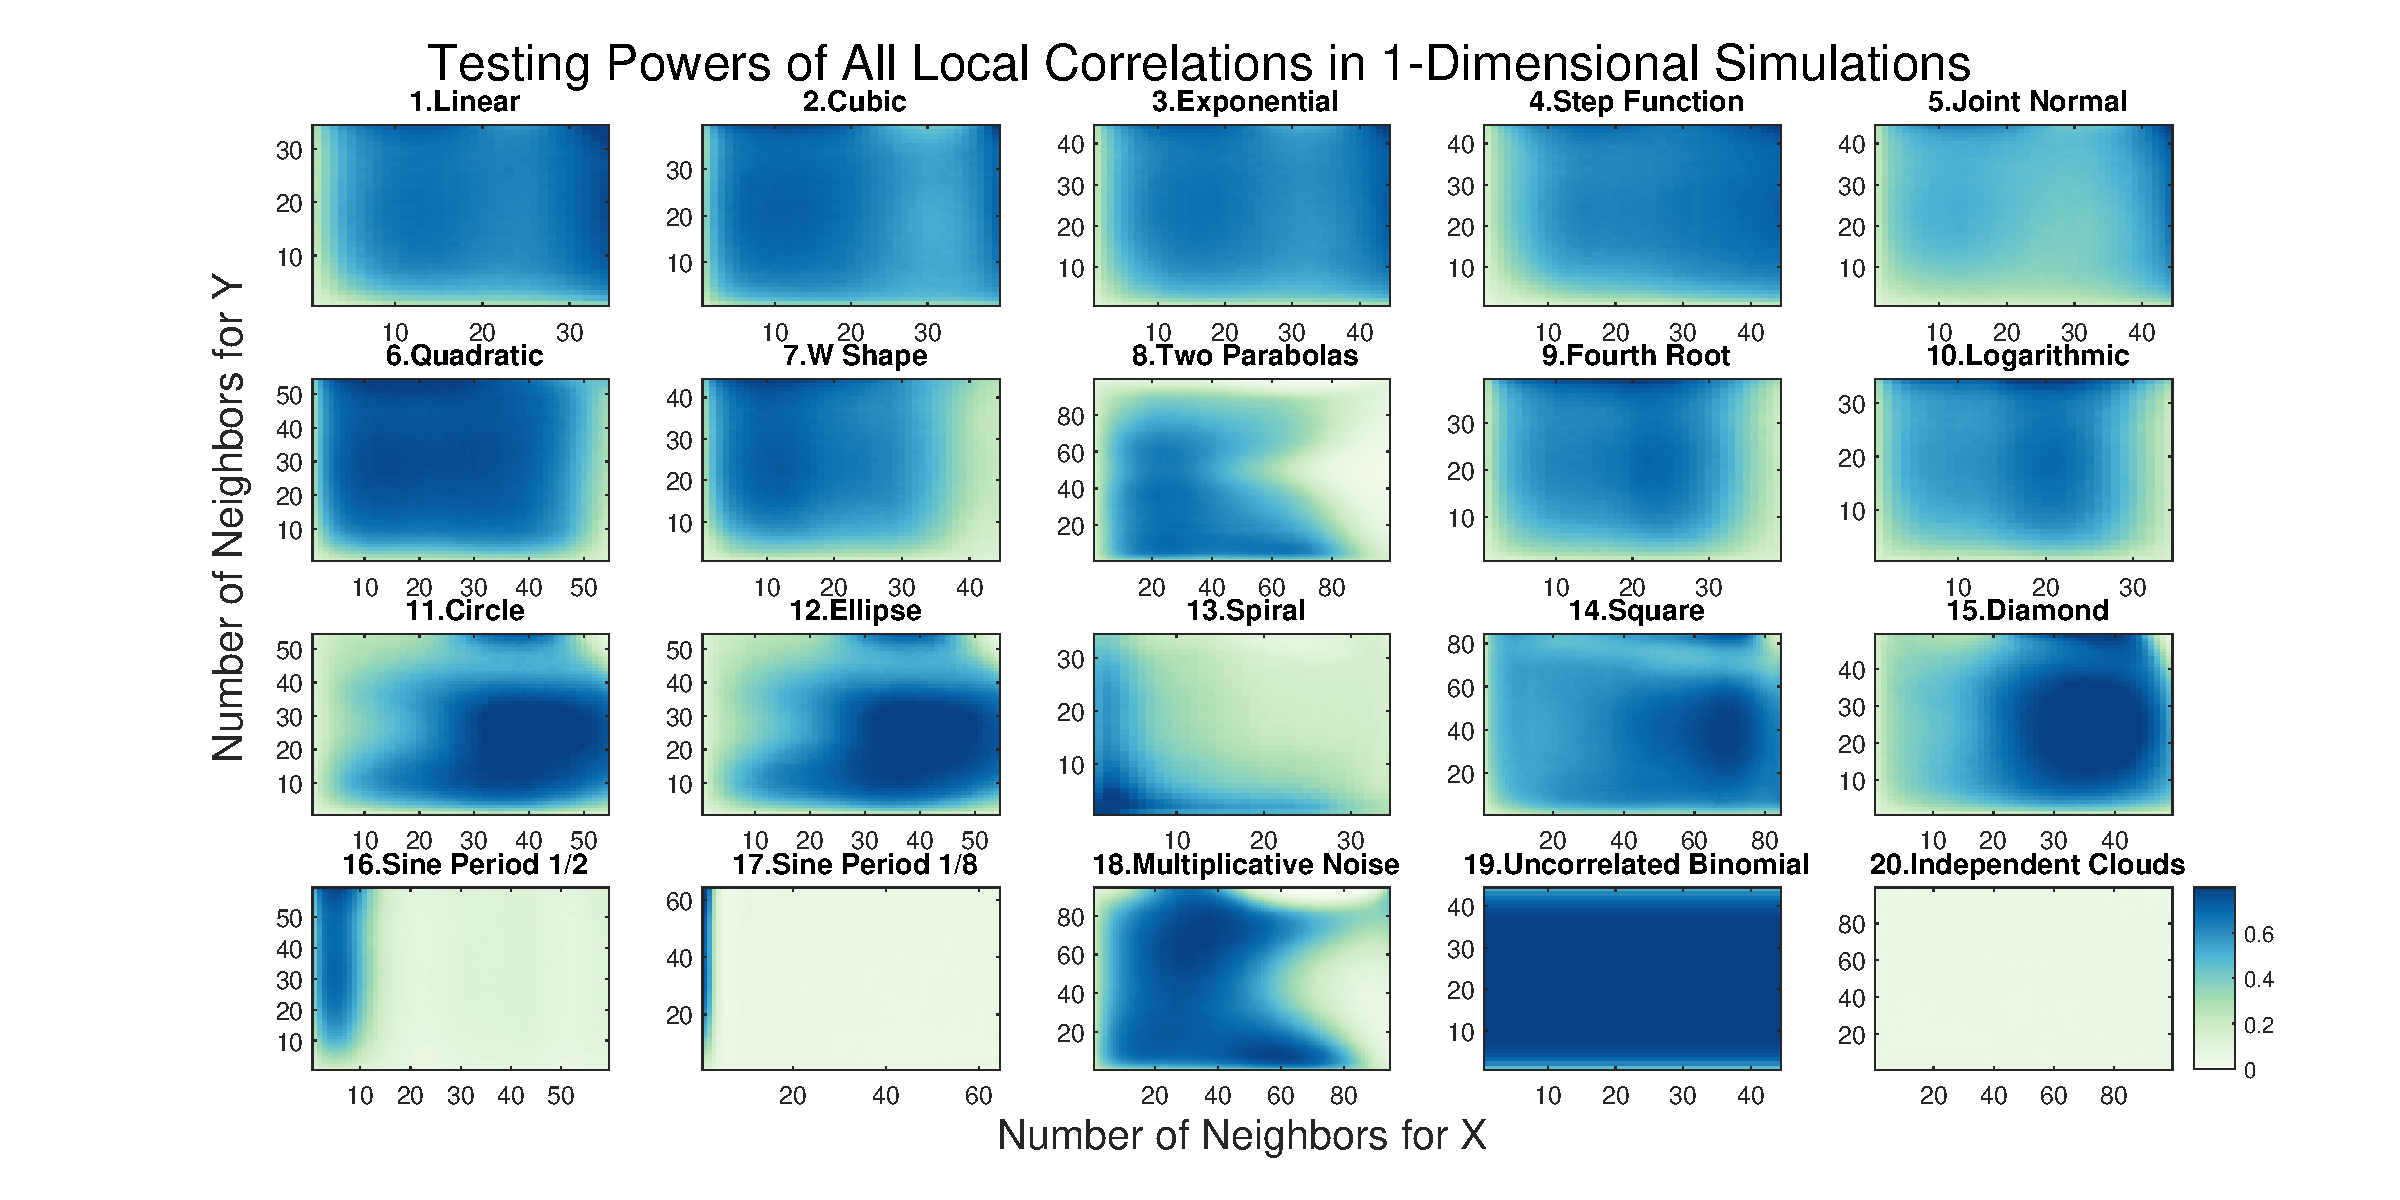
\includegraphics[width=1.0\textwidth]{Figures/Fig2}
\caption{Testing power heat map of local mcorr correlations with respect to number of neighbors in the $1$-dimensional simulations. For each simulation, the dimension is $1$, and the sample size is determined by the power threshold as in figure~\ref{fig:pp}(A).
}
\label{figSim2}
\end{figure}

\section{Performance Profiles}
\label{appen:profiles}
The performance profiles of each method are drawn by the following steps:

Suppose there are $S$ methods and $T$ different problems, and the respective powers are denoted as $\beta_{\alpha}^{t}(s)$ for $s=1,\ldots,S$ and $t=1,\ldots,T$ at a fixed type 1 error $\alpha$. Then the relative performance for each method is defined as follows:
\begin{align*}
performance_{s}(x) &= \frac{1}{T} \sum_{t=1}^{T} \mb{I}((\beta_{\alpha}^{t}(*)-\beta_{\alpha}^{t}(s)) \leq x)
\end{align*}
where $x \in [0,1]$, $\mb{I}$ is the indicator function, and $\beta_{\alpha}^{t}(*) =\max_{s} \{\beta_{\alpha}^{t}(s)\}$ denotes the best testing power in the $t$th problem. Namely $x$ stands for the difference with respect to the best power, and the relative performance of each method equals the proportion of simulations that the method is worse than the best method by no more than $x$. For example, at $x=0.1$, MGC has a relative performance of $0.75$ if and only if there are $15$ out of $20$ simulations that MGC is worse than the best method by no more than $0.1$ in testing power. Note that the performance profiles at $x=0$ stands for the proportion of simulations that the method has the best power; and the curve always increases to $1$ at $x=1$. 

\section{Dependence Measures}
\label{appen:methods}

In this section, we review distance correlation, modified distance correlation, the Mantel test, and the HHG statistic in order. Note that for dcorr / mcorr, we implement them in a slightly different but equivalent way from the original definition.

\subsection{(Global) Distance Correlation}
\label{appen:dcorr}
Given two distance matrices $\tilde{A}$ and $\tilde{B}$ of the sample data $X$ and $Y$, the sample distance covariance is defined by doubly centering the distance matrices:
\begin{equation}
\label{dcovEqu}
dcov(X,Y)=\frac{1}{n^2}\sum_{i,j=1}^{n}a_{ij}b_{ij},
\end{equation}
where $A=H\tilde{A}H$, $B=H\tilde{B}H$ with $H=I_{n}-\frac{J_{n}}{n}$. Then the sample distance variance is defined as
\begin{align*}
dvar(X) &=\frac{1}{n^2}\sum_{i,j=1}^{n}a_{ij}^{2},\\
dvar(Y) &=\frac{1}{n^2}\sum_{i,j=1}^{n}b_{ij}^{2},
\end{align*}
and the sample distance correlation equals
\begin{equation}
\label{dcorrEqu}
dcorr(X,Y)=\frac{dcov(X)}{\sqrt{dvar(X) \cdot dvar(Y)}}.
\end{equation}
Note that the sample means $\bar{a}, \bar{b}$ in Equation~\ref{generalCoef} are automatically $0$.

It is shown in \cite{SzekelyRizzoBakirov2007} that as $n \rightarrow \infty$, $dcorr(X,Y) \rightarrow dcorr(\mb{x},\mb{y}) \geq 0$, where $dcorr(\mb{x},\mb{y})$ denotes the population distance correlation between the underlying random variable $\mb{x}$ and $\mb{y}$. The population distance correlation is defined by the characteristic functions, which is $0$ if and only if $\mb{x}$ and $\mb{y}$ are independent. Thus the sample distance correlation is a consistent statistic for testing independence, i.e., the testing power $\beta_{\alpha}(dcorr(X,Y))$ converges to $1$ as $n$ increases, at any type $1$ error level $\alpha$. Note that all of $dcov, dvar, dcorr$ are always non-negative; and the consistency result assumes finite second moments of $\mb{x}$ and $\mb{y}$, which holds for a family of metrics not limited to the Euclidean distance \cite{Lyons2013}. Also note that the $dcorr$ above is actually the square of distance correlation in \cite{SzekelyRizzoBakirov2007}, but for ease of presentation the square naming is dropped here.

Alternatively, calculating the distance covariance by $A=H\tilde{A}$ and $B=\tilde{B}H$ gives the same statistic as in Equation~\ref{dcovEqu}, i.e., instead of using doubly centered distance matrices, it is the same to singly center one distance matrix by row and the other distance matrix by column. Then dcorr by singly centered distance matrices has the same testing power as the original dcorr, because distance covariance is equivalent to distance correlation in the permutation test (note that the actual dcorr statistic by single centering is different from the original dcorr, as using single centering changes the distance variances).

In our implementation of global / local dcorr, we always use singly centered distance matrices rather than doubly centered distance matrices. Although they are equivalent for the testing power of global dcorr, our alternative implementation improves the testing power of local dcorr and MGC. This is because the ranking information of $\tilde{A}$ and $\tilde{B}$ are better preserved in singly centered distance matrices, so that MGC is more effective in excluding far-away points that exhibit insignificant dependency.

\subsection{(Global) Modified Distance Correlation}
\label{appen:mcorr}
In case of high-dimensional data where the dimension $d_{x}$ or $d_{y}$ increases with the sample size $n$, the sample distance correlation may no longer be appropriate. For example, even for independent Gaussian distributions, $dcorr(X,Y) \rightarrow 1$ as $d_{x}, d_{y} \rightarrow \infty$, which may severally impair the testing power of sample dcorr in high-dimensional simulations.

The modified distance correlation is proposed in \cite{SzekelyRizzo2013a} to tackle the bias of sample dcorr. Denote the Euclidean distance matrices as $\tilde{A}$ and $\tilde{B}$, the doubly centered distance matrices as $\hat{A}$ and $\hat{B}$, the modified distance covariance is defined as
\begin{equation}
\label{mcovEqu}
mcov(X,Y)=\frac{n}{(n-1)^2(n-3)}(\sum_{i \neq j}^{n}a_{ij}b_{ij}-\frac{2}{n-2}\sum_{j=1}^{n}a_{jj}b_{jj}),
\end{equation}
where $A$ modifies the entries of $\hat{A}$ by
\[a_{ij} = \left\{
  \begin{array}{lr}
    \hat{a}_{ij}-\frac{\tilde{a}_{ij}}{n}, & \mbox{ if } i \neq j, \\
    \frac{n\sum_{i}\tilde{a}_{ij}-\sum_{i,j}\tilde{a}_{ij}}{n^2}, &\mbox{ if } i = j,
  \end{array}
\right.
\]
and so is $B$. Then $mvar(X)$ and $mvar(Y)$ can be similarly defined. 

If $mvar(X) \cdot mvar(Y) \leq 0$, the modified distance correlation is set to $0$ (negativity can only occur when $n\leq 2$, equality can only happen in some special cases); otherwise it is defined as
\begin{equation}
\label{mcorrEqu}
mcorr(X,Y)=\frac{mcov(X,Y)}{\sqrt{mvar(X) \cdot mvar(Y)}}.
\end{equation}

It is shown in \cite{SzekelyRizzo2013a} that $mcorr(X,Y)$ is an unbiased estimator of the population distance correlation $dcorr(\mb{x},\mb{y})$ for all $d_{x}, d_{y}, n$; and mcorr is approximately normal even if $d_{x},d_{y} \rightarrow \infty$. Thus it is a consistent statistic for testing independence, but may work better than dcorr under high-dimension dependencies. 

Similar to the alternative implementation of dcorr, we can also use singly centered distance matrices for $\hat{A}$ and $\hat{B}$ in defining mcorr, which does not alter the theoretical advantages of original mcorr. We further set $A_{ii}=B_{ii}=0$ for all $i$, which simplifies the expression of mcorr and is asymptotically equivalent for the testing purpose. %Also note that when there exists repeating points, it is necessary to set $a_{ij}=a_{jj}$ for repeating points during global/local mcorr computation, or exclude repeating observation before-hand, otherwise the diagonal adjustment of mcorr may lose its effect for adjusting high-dimensional bias.

\subsection{(Global) Mantel Test}
\label{appen:mantel}
Given the Euclidean distance matrices $\tilde{A}$ and $\tilde{B}$, the Mantel coefficient \cite{Mantel1967} is defined as 
\begin{equation}
Mantel(X,Y)=\frac{\sum_{i \neq j}^{n}(a_{ij}-\bar{a})(b_{ij}-\bar{b})}{\sqrt{\sum_{i \neq j}^{n}(a_{ij}-\bar{a})^2 \sum_{i \neq j}^{n}(b_{ij}-\bar{b})^2}},
\end{equation}
where $A=\tilde{A}$, $B=\tilde{B}$, $\bar{a}=\frac{1}{n(n-1)}\sum_{i \neq j}^{n}(a_{ij})$ and similarly for $\bar{b}$. Intuitively, the Mantel coefficient treats the two distance matrices (excluding the diagonals) as two observation vectors, and calculates the Pearson's correlation between them; then the Mantel test is carried out by the permutation test.

Unlike distance correlation and HHG, the Mantel test is not consistent against all dependent alternatives, but it has been a very popular method in biology and ecology due to its simplicity. It is clear from figure~\ref{fig:nD} that global Mantel is sub-optimal and appears to be not consistent for many dependencies, yet MGC by Mantel achieves comparable performances as other variants of MGC, which implies that MGC$\{$Mantel$\}$ may be consistent against most, if not all dependent alternatives.

\subsection{Heller, Heller \& Gorfine (HHG)}
\label{appen:hhg}
The HHG statistic applies Pearson's chi-square test to ranks of distances within each column, and is shown to be better than many global tests including dcorr under common nonlinear dependencies in \cite{GorfineHellerHeller2012, HellerGorfine2013}. Like dcorr and mcorr, HHG is distance-based and consistent, but not in the form of the general correlation coefficient; and like our MGC, it makes use of the rank information, but in a distinct manner.

Given the Euclidean distance matrices $\tilde{A}=[\tilde{a}_{ij}]$ and $\tilde{B}=[\tilde{b}_{ij}]$, we denote
\begin{align*}
H_{11}(i,j) &= \sum_{q=1,q\neq i,j}^{n}I(\tilde{a}_{ik} \leq \tilde{a}_{ij})I(\tilde{b}_{ik} \leq \tilde{b}_{ij}) \\
H_{12}(i,j) &= \sum_{q=1,q\neq i,j}^{n}I(\tilde{a}_{ik} \leq \tilde{a}_{ij})I(\tilde{b}_{ik} > \tilde{b}_{ij}) \\
H_{21}(i,j) &= \sum_{q=1,q\neq i,j}^{n}I(\tilde{a}_{ik} > \tilde{a}_{ij})I(\tilde{b}_{ik} \leq \tilde{b}_{ij}) \\
H_{22}(i,j) &= \sum_{q=1,q\neq i,j}^{n}I(\tilde{a}_{ik} > \tilde{a}_{ij})I(\tilde{b}_{ik} > \tilde{b}_{ij}),
\end{align*}
and the HHG statistic is defined as
\begin{align*}
HHG(X,Y) &= \sum_{i=1,j\neq i}^{n} \frac{(n-2)(H_{12}(i,j)H_{21}(i,j)-H_{11}(i,j)H_{22}(i,j))^2}{H_{1 \cdot}(i,j)H_{2 \cdot}(i,j)-H_{\cdot 1}(i,j)H_{\cdot 2}(i,j)},
\end{align*}
where $H_{1 \cdot}=H_{11}+H_{12}$, $H_{2 \cdot}=H_{21}+H_{22}$, $H_{\cdot 1}=H_{11}+H_{21}$, and $H_{\cdot 2}=H_{12}+H_{22}$. It is clear that HHG is structurally different from dcorr / mcorr / Mantel, cannot be conveniently expressed by Equation~\ref{generalCoef}, and there is no direct extension of local correlation to HHG.

The permutation test using the HHG statistic is consistent against all dependent alternatives. In our numerical simulations, HHG falls a bit short when testing against high-dimensional and noisy linear dependencies, but is often more advantageous than global correlations under nonlinear dependencies, which makes it a strong competitor in general. 

\section{MGC Algorithms and Testing Procedures}
\label{appen:tests}
In this section we elaborate on the algorithms for computing local correlation and MGC, as well as their testing procedures in simulations and real data experiment. 

For any general correlation coefficient in Equation~\ref{generalCoef}, the local correlations can be directly implemented by Equation~\ref{localCoef} through sorting the distance matrices column-wise and plugging in the appropriate $a_{ij}, b_{ij}$. Note that among all local correlations, it suffices to exclude $\G_{1l}$ and $\G_{k1}$ for testing: since $\G_{1l}=\G_{k1}=\G_{11}$, they do not include any neighbor other than each observation itself, merely count the diagonal terms in the distance matrices, and are not meaningful for the testing purpose. Also note that we use minimal ranks in sorting when ties occur, which indexes all local correlations more conveniently than breaking ties randomly or using average / max ranks.

Five algorithms are presented in section~\ref{appen:algorithms}: given the choice of a global correlation coefficient, algorithm~\ref{alg1} computes one local correlation coefficient at a given $(k,l)$; then algorithm~\ref{alg2} shows how to compute all local correlations simultaneously; algorithm~\ref{alg3} estimates the testing powers of all local statistics based on a given joint distribution or multiple pairs of data, which can be used to estimate the powers of all local tests / MGC and thus the optimal scale for MGC; algorithm~\ref{alg4} computes the p-values of all local correlation by the random permutation test; and algorithm~\ref{alg5} approximates the optimal scale for MGC based on the p-values of all local correlations, and outputs the approximated p-value of MGC. More detailed discussions regarding the optimal scale approximation is offered in section~\ref{appen:diss}.

\subsection{Algorithms}
\label{appen:algorithms}
All algorithms are implemented in Matlab and R with the pseudo-code shown below. For ease of presentation, we assume there are no repeating data and take dcorr as the global corr in the pseudo-code.

Algorithm~\ref{alg1} shows a straightforward computation of one local correlation coefficient, which requires $O(n^2)$ once the rank information is provided. This is suitable for MGC computation when the optimal local scale is known or already estimated. But using algorithm~\ref{alg1} to compute all local correlations would require iterating through all possible neighborhoods $(k,l)$, which takes $O(n^4)$ and would make the optimal scale estimation computationally inefficient. 

To facilitate the optimal scale estimation, algorithm~\ref{alg2} provides a fast method to compute all local correlations in $O(n^2)$. An important observation is that each product $a_{ij}b_{ij}$ is included in $\G_{kl}$ if and only if $(k,l)$ satisfies $k\leq rank(a_{ij})$ and $l\leq rank(b_{ij})$, so it suffices to iterate through $a_{ij}b_{ij}$ for $i,j=1,\ldots,n$, and add the product simultaneously to all $\G_{kl}$ whose scales are no more than $(rank(a_{ij}),rank(b_{ij}))$. However, accessing and adding multiple $\G_{kl}$ at the same time is not computationally efficient; instead, for each product, we only add it to $\G_{kl}$ at $(k,l)=(rank(a_{ij}),rank(b_{ij}))$ (so only one local scale is accessed for each operation), iterate through all products for $i,j=1,\ldots,n$, then add up adjacent $\G_{kl}$ for $k,l=1,\ldots,n$. Thus all local correlations can be computed in $O(n^2)$, which has the same running time complexity as the global distance correlation. There are two additional overheads: sorting the distance matrices column-wise takes $O(n^2 \log n)$, and properly centering the distance matrices takes $O(n^2)$. 

Algorithm~\ref{alg3} computes the testing powers of all local correlations by repeated simulating samples generated from the joint distribution $f_{xy}$. Sample data under the null and the alternative are repeatedly generated for $r$ Monte-Carlo replicates, and algorithm~\ref{alg2} is applied to compute the sample local correlations under the null and the alternative. Then the testing power at each local correlation can be estimated, and the MGC optimal scale can be found by maximizing the powers. This algorithm is also applicable if there exists multiple pairs of data with unknown model but similar dependency structure, then the alternative statistic can be computed from each data pair while the null statistic can be computed from each data pair under permutation.

Algorithm~\ref{alg4} computes the p-values of all local correlation by the permutation test with $r$ random permutations. Both algorithm~\ref{alg3} and ~\ref{alg4} takes $O(rn^2 \log n)$, and can be used to compute the power / p-value of MGC once the optimal scale is determined, or the power / p-value of any global correlation by excluding the respective local indexing.

Algorithm~\ref{alg5} approximates the optimal scale $(k^{*},l^{*})$ from the p-values of all local correlations, and outputs the approximated MGC p-value. This is necessary for testing on one pair of data with unknown model, since algorithm~\ref{alg3} may no longer be used. Conceptually, the algorithm first searches for a set of ``valid'' adjacent rows $\K=\{k_{1},k_{1}+1,\ldots,k_{2}-1,k_{2}\}$ such that the median p-value of $\{p_{kl},k \in \K, l=2,\ldots,n\}$ is no larger than $\alpha /(n-1) * |\K|$, otherwise we take $\K=\{n\}$; and similarly determine the set of valid columns $\LL$. Once $\K$ and $\LL$ are determined, the optimal scale $(k^{*},l^{*})$ is found by the scale that minimizes the p-value within $\{p_{kl},k \in \K, l \in \LL\}$. Clearly if the majority p-values of all local correlations are less than $\alpha$, then $\K=\LL=\{1,\ldots,n\}$, and the optimal scale equals the scale that minimizes the p-values among all local correlations; if there is no valid rows and columns, then MGC takes the largest scale and equals the global correlation. Note that the actual algorithm is a simpler version of the above description: instead of considering all possible sets of rows and check the validity, we limit the check to the most likely set of rows, by first looking for the row scale of the smallest p-value, then including all adjacent rows whose minimal p-value on the row is no larger than $\alpha$; similarly for the set of columns.

\begin{algorithm}
\caption{Local Correlation Computation for One Scale}
\label{alg1}
\begin{algorithmic}[1]
\Statex Input: A pair of distance matrices $(\tilde{A},\tilde{B}) \in \Real^{n \times n} \times \Real^{n \times n}$, and the given local scale $(k,l) \in \Real \times \Real$.
\Statex Output: The local correlation coefficient $\G_{kl} \in [-1,1]$ at the given $(k,l)$.
\Function{LocalCorr}{$\tilde{A}$,$\tilde{B}$,$k$,$l$}
\State initialize $\G^{kl}$, $V^{A}_{k}$, $V^{B}_{l}$, $E^{A}_{k}$, $E^{B}_{l}$ as $0$.
\Linefor{$Z:=A,B$}{$R^{Z}=\textsc{Sort}(\tilde{Z})$} \Comment{column-wise sorting and assume no ties}
\Linefor{$Z:=A,B$}{$Z=\textsc{Center}(\tilde{Z})$} \Comment{proper centering of the distance matrices}
\For{$i,j=1,\ldots,n$}
\State $\G_{kl}=\G_{kl}+A_{ij}B_{ij}\mb{I}(R^{A}_{ij} \leq k)\mb{I}(R^{B}_{ij} \leq l)$ \Comment{store local distance covariance}
\State $V^{A}_{k}=V^{A}_{k}+A_{ij}^2\mb{I}(R^{A}_{ij} \leq k)$ \Comment{store local distance variance for $X$}
\State $V^{B}_{l}=V^{B}_{l}+B_{ij}^2\mb{I}(R^{B}_{ij} \leq l)$ \Comment{store local distance variance for $Y$}
\State $E^{A}_{k}=E^{A}_{k}+A_{ij}\mb{I}(R^{A}_{ij} \leq k)$ \Comment{store the sample means}
\State $E^{B}_{l}=E^{B}_{l}+B_{ij}\mb{I}(R^{B}_{ij} \leq l)$
\EndFor

\State $\G_{kl}=\left(\G_{kl}-E^{A}_{k}E^{B}_{l}/n^2\right)/\sqrt{\left(V^{A}_{k}-{E^{A}_{k}}^2/n^2\right) \left(V^{B}_{l}-{E^{B}_{l}}^2/n^2\right)}$ \Comment{normalize the local covariances}

\EndFunction
\end{algorithmic}
\end{algorithm}

\begin{algorithm}
\caption{$O(n^2 \log n)$ Algorithm for Computing All Local Correlations}
\label{alg2}
\begin{algorithmic}[1]
\Statex Input: A pair of distance matrices $(\tilde{A},\tilde{B}) \in \Real^{n \times n} \times \Real^{n \times n}$.
\Statex Output: All local correlation coefficients $\G_{kl} \in [-1,1]^{n \times n}$ for $k,l=1,\ldots,n$.
\Function{LocalCorr}{$\tilde{A}$,$\tilde{B}$}
\State initialize $\G$ as a zero matrix of size $n \times n$; $V^{A}$, $V^{B}$, $E^{A}$, $E^{B}$ as zero vectors of size $n$.
\Linefor{$Z:=A,B$}{$R^{Z}=\textsc{Sort}(\tilde{Z})$} 
\Linefor{$Z:=A,B$}{$Z=\textsc{Center}(\tilde{Z})$} 
\For{$i,j=1,\ldots,n$}
\State $k=R^{A}_{ij}$
\State $l=R^{B}_{ij}$
\State $\G_{kl}=\G_{kl}+A_{ij}B_{ij}$
\State $V^{A}_{k}=V^{A}_{k}+A_{ij}^2$
\State $V^{B}_{l}=V^{B}_{l}+B_{ij}^2$
\State $E^{A}_{k}=E^{A}_{k}+A_{ij}$ 
\State $E^{B}_{l}=E^{B}_{l}+B_{ij}$
\EndFor
\Statex \Comment{the next two for loops with respect to the scales guarantee the computation of all local covariance / variance in $O(n^2)$}
\For{$k=1,\ldots,n-1$}
\State $\G_{1, k+1}=\G_{1, k}+\G_{1, k+1}$
\State $\G_{k+1,1}=\G_{k+1,1}+\G_{k+1,1}$
\Linefor{$Z:=A,B$}{$V^{Z}_{k+1}=V^{Z}_{k}+V^{Z}_{k+1}$} 
\Linefor{$Z:=A,B$}{$E^{Z}_{k+1}=E^{Z}_{k}+E^{Z}_{k+1}$} 
\EndFor

\For{$k,l=1,\ldots,n-1$}
\State $\G_{k+1,l+1}=\G_{k+1,l}+\G_{k,l+1}+\G_{k+1,l+1}-\G_{k,l}$
\EndFor

\For{$k,l=1,\ldots,n$} \Comment{normalize all local covariances}
\State $\G_{kl}=\left(\G_{kl}-E^{A}_{k}E^{B}_{l}/n^2\right)/\sqrt{\left(V^{A}_{k}-{E^{A}_{k}}^2/n^2\right) \left(V^{B}_{l}-{E^{B}_{l}}^2/n^2\right)}$
\EndFor
\EndFunction
\end{algorithmic}
\end{algorithm}

\begin{algorithm}
\caption{Testing Powers Computation for All Local Correlations}
\label{alg3}
\begin{algorithmic}[1]
\Statex Input: A joint distribution $f_{xy}$, the sample size $n$, the number of MC replicates $r$, and the type $1$ error level $\alpha$.
\Statex Output: The power matrix $\beta_{\alpha} \in [0,1]^{n \times n}$ for all local correlations, and the MGC optimal scale $(k^{*},l^{*}) \in \Real \times \Real$.
\Function{TestingPowers}{$f_{xy}$,$n$, $r$,$\alpha$} 
\For{$j=1,\ldots,r$} 
\Linefor{$i:=[n]$}{$(X^{1}_{i},Y^{1}_{i}) \stackrel{iid}{\sim} f_{xy}$} \Comment{generate dependent samples}
\Linefor{$i:=[n]$}{$X^{0}_{i} \stackrel{iid}{\sim} f_{x}$} \Comment{generate independent samples}
\Linefor{$i:=[n]$}{$Y^{0}_{i} \stackrel{iid}{\sim} f_{y}$} 
\Linefor{$Z:=A,B$}{$\tilde{Z}^{1}=\textsc{Dist}(Z^{1})$} \Comment{the distance matrices under the alternative}
\Linefor{$Z:=A,B$}{$\tilde{Z}^{0}=\textsc{Dist}(Z^{0})$} \Comment{the distance matrices under the null}
\State $\G_{kl}^{1}[j]=\textsc{LocalCorr}(\tilde{A}^{1},\tilde{B}^{1})$ \Comment{calculate all local correlations under the alternative} 
\State $\G_{kl}^{0}[j]=\textsc{LocalCorr}(\tilde{A}^{0},\tilde{B}^{0})$ \Comment{calculate all local correlations under the null} 
\EndFor

\For{$k,l=1,\ldots,n$}
\State $c_{\alpha}=\textsc{Cdf}_{1-\alpha}(\G^{0}_{kl}[j],j \in [r])$ \Comment{get the critical value by the empirical cumulative distribution under the null at each scale}
\State $\beta_{\alpha}^{kl}=\sum_{j=1}^{r}(\G^{1}_{kl}[j]>c_{\alpha}) / r$ \Comment{estimate the power}
\EndFor
\State $(k^{*},l^{*})=\arg\max(\beta_{\alpha}^{kl})$ \Comment{find the optimal local scale}
\EndFunction
\end{algorithmic}
\end{algorithm}

\begin{algorithm}
\caption{P-value Computation for All Local Correlations}
\label{alg4}
\begin{algorithmic}[1]
\Statex Input: A pair of distance matrices $(\tilde{A},\tilde{B}) \in \Real^{n \times n} \times \Real^{n \times n}$, the number of permutations $r$.
\Statex Output: The p-value matrix $P \in [0,1]^{n \times n}$ for all local distance correlations.
\Function{PermutationTest}{$\tilde{A}$,$\tilde{B}$,$r$}
\State $\G_{kl}=\textsc{LocalCorr}(\tilde{A},\tilde{B})$ \Comment{calculate the observed local correlations}
\For{$j=1,\ldots,r$}
\State $\pi=\textsc{RandPerm}(n)$ \Comment{generate a random permutation of size $n$}
\State $\G_{kl}^{0}[j]=\textsc{LocalCorr}(\tilde{A},\tilde{B}(\pi,\pi))$ \Comment{calculate the permuted test statistics}
\EndFor

\For{$k,l=1,\ldots,n$}
\State $P_{kl}=\sum_{j=1}^{r}(\G_{kl}<\G^{0}_{kl}[j])/r$ \Comment{get the p-value at each local scale}
\EndFor
\EndFunction
\end{algorithmic}
\end{algorithm}

\begin{algorithm}
\caption{Optimal Local Scale Approximation by P-values}
\label{alg5}
\begin{algorithmic}[1]
\Statex Input: The p-value matrix $P \in \Real^{n \times n}$ of all local distance correlations, the type $1$ error level $\alpha$.
\Statex Output: The approximated MGC optimal scale $(k^{*},l^{*})$, and the approximated MGC p-value $p$.
\Function{MGCScaleVerify}{$P$, $\alpha$}
\State $\K=\textsc{VerifyRow}(P,\alpha)$ \Comment{search for a set of valid row indices}
\State $\LL=\textsc{VerifyRow}(P\T,\alpha)$ \Comment{search for a set of valid column indices}
\State $[k^{*},l^{*}]=\arg\min_{\left\{k \in \K, l \in \LL\right\}} P_{kl}$ \Comment{find the optimal scale within the valid range}
\State $p=P_{k^{*}l^{*}}$
\EndFunction
\end{algorithmic}

\begin{algorithmic}[1]
\Statex
\Statex Input: Same as \textsc{MGCScaleVerify}.
\Statex Output: The indices of valid rows.
\Function{VerifyRow}{$P$, $\alpha$}
\State initialize $\K$ as an empty set
\State $[k^{*},l^{*}]=\arg\min_{k, l} \{P_{kl},k,l=2,\ldots,n\}$
\For{$k=k^{*},\ldots,2$} \Comment{check all row scales no larger than $k^{*}$}
\If{$\min\{P_{kl},l=2,\ldots,n\}>\alpha$}
\State break
\EndIf
\State $\K=[k,\K]$
\EndFor
\For{$k=k^{*}+1,\ldots,m$} \Comment{check all row scales larger than $k^{*}$}
\If{$\min\{P_{kl},l=2,\ldots,n\}>\alpha$}
\State break
\EndIf
\State $\K=\{\K,k\}$
\EndFor
\If{$\textsc{Median}(P_{kl},k \in \K, l=2,\ldots,n) > \alpha * \frac{|\K|}{n-1}$}
\State $\K=\{n\}$ \Comment{take the largest scale if the median p-value is not sufficiently small}
\EndIf
\EndFunction
\end{algorithmic}
\end{algorithm}

\subsection{Discussions of Optimal Scale Estimation}
\label{appen:diss}
To evaluate MGC in simulations or real data, the optimal scale for MGC always needs to be estimated first. Algorithm~\ref{alg3} computes the testing powers of all local correlations for known model, so the optimal scale $(k^{*},l^{*})$ can be directly estimated by maximizing the testing powers (if there are more than one optimal scales, one may pick the scale that maximizes the mean difference of the test statistic under the null and the alternative). Once the optimal scale is determined, the testing power of MGC under the given model can be quickly determined by algorithm~\ref{alg3}, and its p-value for testing on a particular pair of data can be determined by algorithm~\ref{alg4}.

If there is only one pair of data $(X,Y)$ with unknown distributions, we have to approximate the optimal scale by algorithm~\ref{alg5}. It makes use of Bonferroni correction to separately verify the set of rows and columns, which guarantees the false positive rate to be no higher than $\alpha$; otherwise the scale is set to the largest, which guarantees the approximated MGC is at least as powerful as the global correlation. Still, algorithm~\ref{alg5} is a heuristic approach to approximate the optimal local scale, which does not guarantee the optimal local correlation to be always correctly identified.

%As an additional note, for any test statistic, the power of the permutation-based test (algorithm~\ref{algPerm}) is equivalent to the simulated testing power from algorithm~\ref{algPower}, because the permuted sample pairs in algorithm~\ref{algPerm} are independent from each other and follow the same marginal distributions as the independent sample pairs in algorithm~\ref{algPower}. Furthermore, choosing a fair alternative is an important issue for evaluating the testing power, as discussed in \cite{RamdasEtAl2015}.

To better justify algorithm~\ref{alg5}, we compare the estimated MGC power by algorithm~\ref{alg5} to the true MGC power by algorithm~\ref{alg3}, with the global mcorr and HHG as benchmarks. For each type of dependency in the simulation section, we generate $1$,$000$ pairs of dependent data by the same low- and high-dimensional settings as in figure~\ref{fig:pp}(A)(C); and for each pair of data, all local p-values are calculated by $1$,$000$ random permutations. By using the true optimal scale (from the simulation section) consistently for each data pair, the true MGC p-value can be computed; by using algorithm~\ref{alg5} to approximate the optimal scale for each pair of data separately, the estimated MGC p-value can be computed; and the p-values of global mcorr and HHG can also be derived. The null is rejected when the p-value is less than $0.05$, and the power equals the percentage of correct rejection. Based on the powers of true MGC / estimated MGC / mcorr / HHG shown in figure~\ref{figSimPerm}, we observe that although the estimated MGC power by algorithm~\ref{alg5} can be lower than the true MGC power, it is almost always better than global mcorr and HHG, and combines the better performance of the two benchmarks. 

\begin{figure}[htbp]
\centering
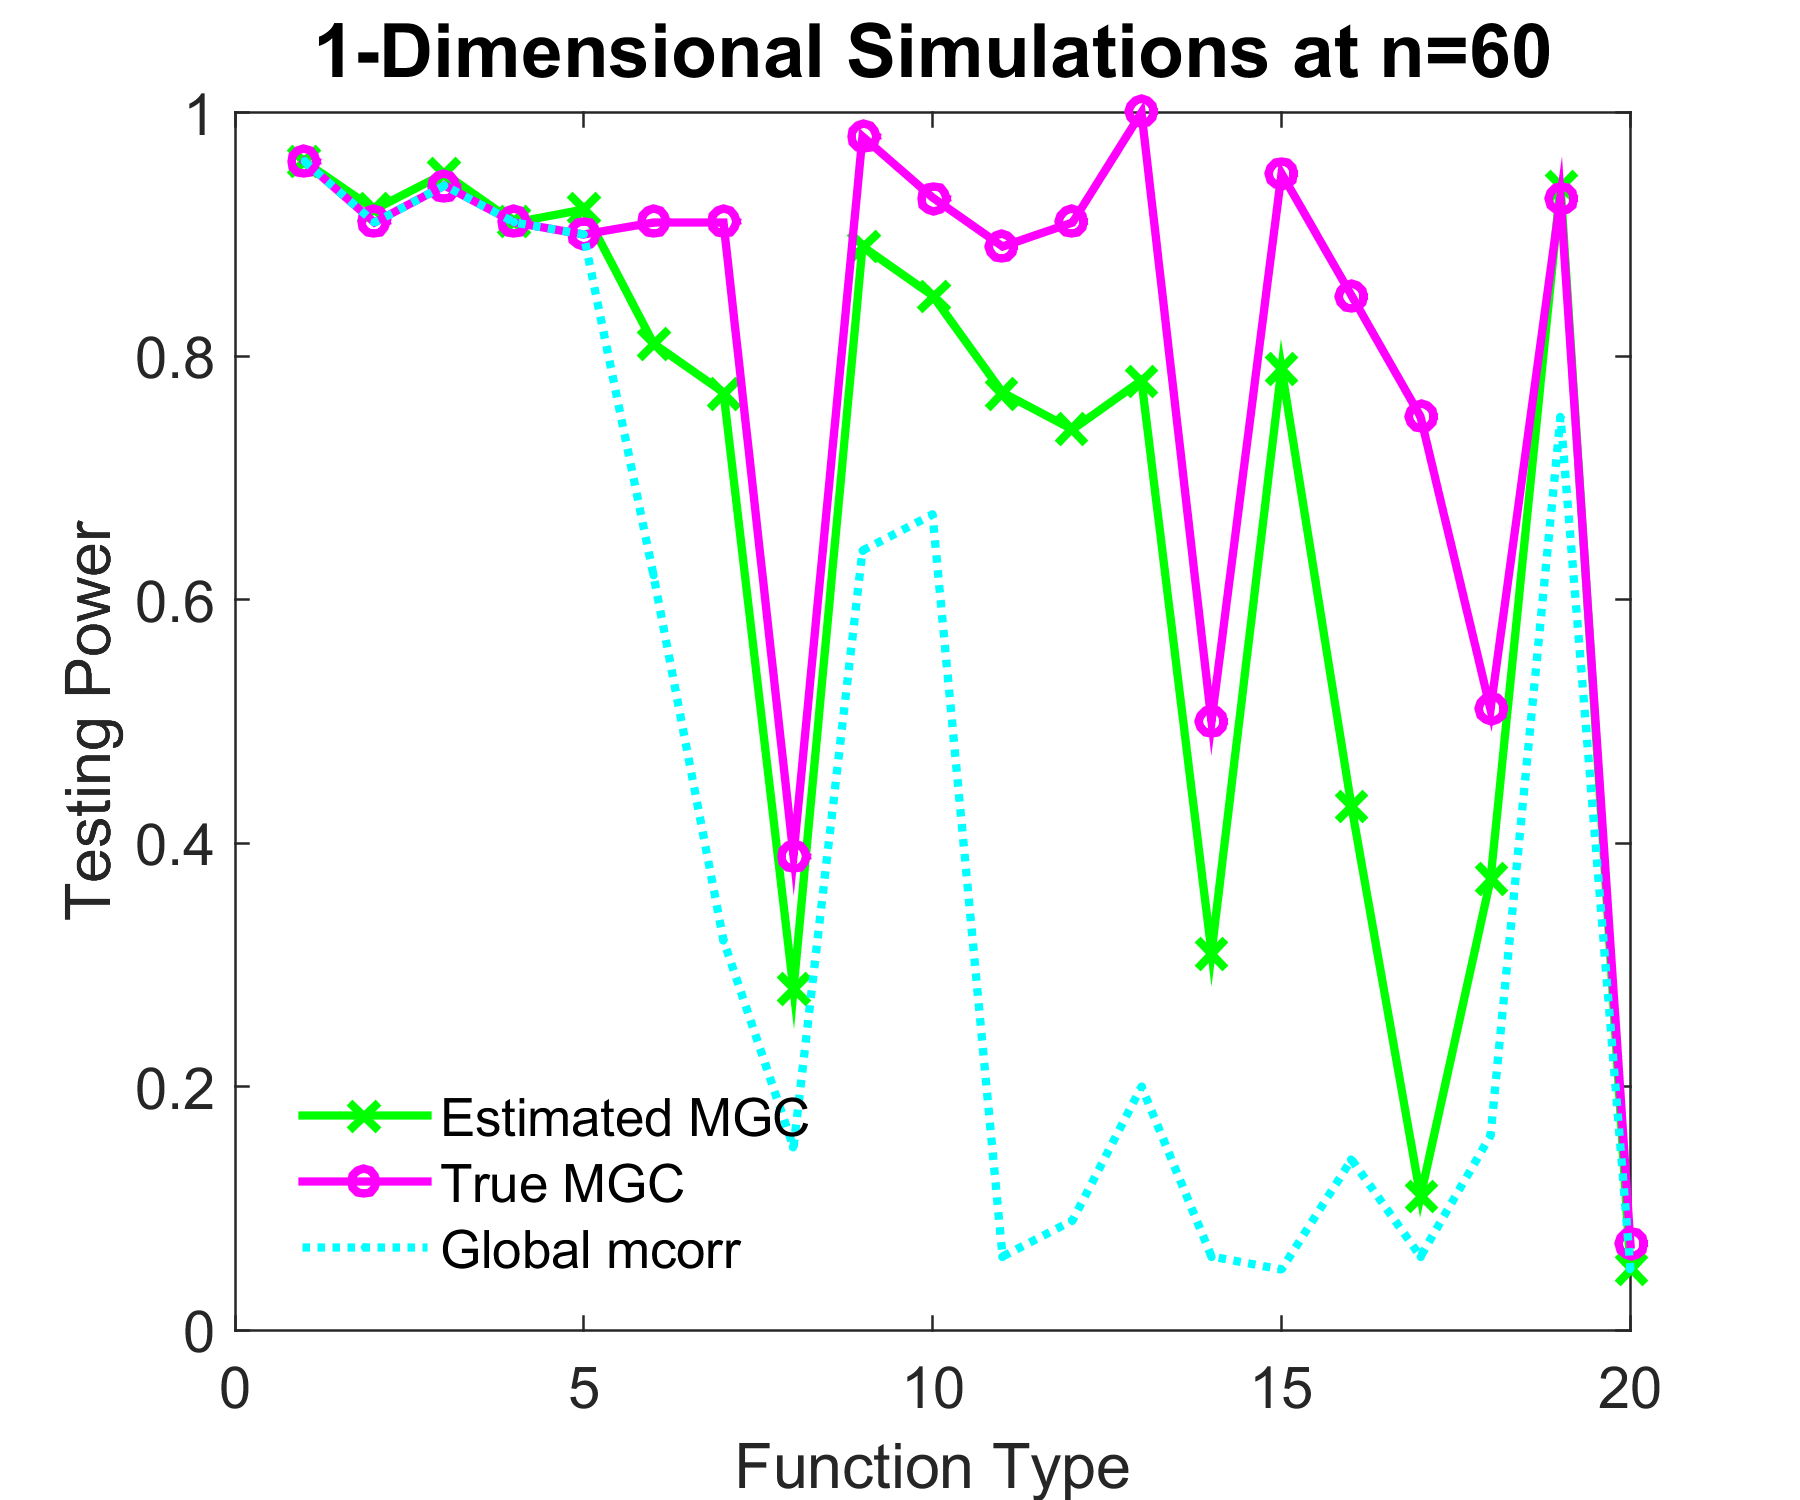
\includegraphics[width=0.45\textwidth]{Figures/Fig9}
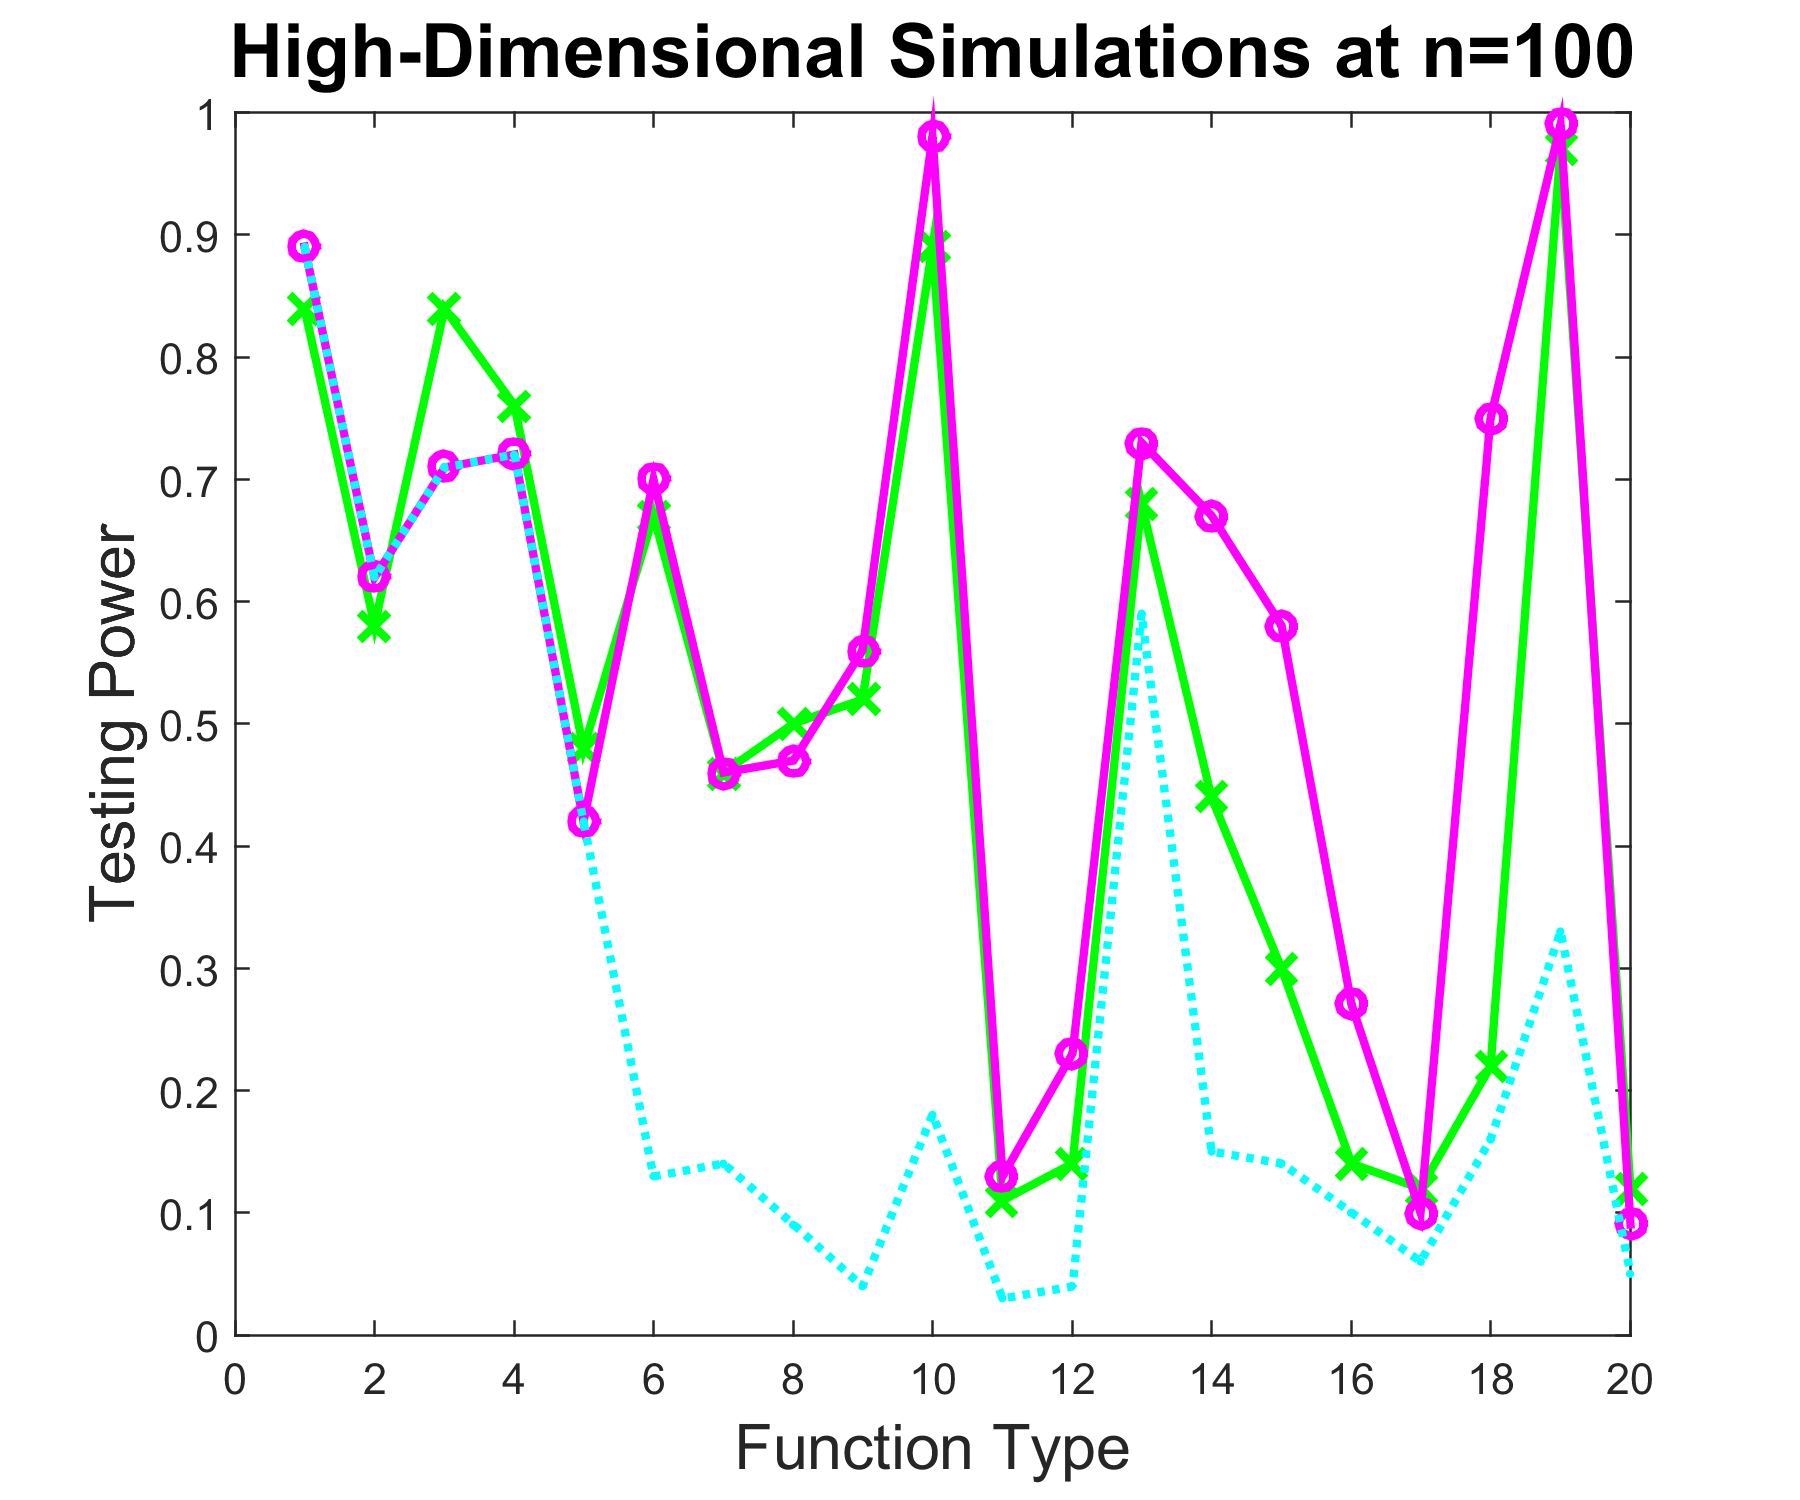
\includegraphics[width=0.45\textwidth]{Figures/Fig10}
\caption{Comparing estimated MGC power to true MGC power, for the $1$-dimensional and high-dimensional simulations. For the $1$-dimensional simulations, $d_{x}=1$ and the sample size is chosen by the power threshold $0.8$ as in figure~\ref{fig:pp}(A); for the high-dimensional simulations, $n=100$ and the dimension is chosen by the power threshold $0.5$ as in figure~\ref{fig:pp}(C). The estimated MGC power by the approximated optimal scale is almost always better than global mcorr and HHG, combines the better performance of the two benchmarks, is quite close to the true MGC power, and does not inflate false signals.} 
\label{figSimPerm}
\end{figure}

Note that it is tempting to directly use the optimal scale that minimizes all local p-values without the validation by algorithm~\ref{alg5}, or generate random samples based on the given data pair and use algorithm~\ref{alg3} by bootstrap. However, both approaches are biased such that the false positive rate will be higher than the type $1$ error in the absence of dependency. This is because for a given pair of data, a non-optimal scale can happen to have a significant p-value, which may be falsely identified as optimal if we directly minimize all local p-values. Those erroneous scales often still exist after a straightforward re-sampling, so random samples have the same problem. More investigations into the bias and better methods for searching the optimal scale are two worthwhile directions for future works.

%This problem does not exist, if we know the underlying true model, or has multiple pairs of training data from the same model that are independent of the testing pair. In case of a known model, we already showed in the simulations that the theoretical MGC power can be achieved without any inflation of the false positive rate, once an optimal scale is determined. Alternatively, if additional data are available, or the full data set is too large such that sub-sampling is necessary for data analysis, we can use / sub-sample multiple training data for optimal scale estimation based on maximizing the sum of p-values of all local correlations, then use the optimal scale on the testing data for p-value calculation; the alternative approach also achieve the theoretical MGC power without bias.

\section{Proofs}
\label{appen:proofs}
\begin{appThm}
Suppose for given $f_{xy}$ and $\alpha$, $\beta_{\alpha}(\G) \rightarrow 1$ as $n \rightarrow \infty$, then $\beta_{\alpha}(\G^{*}) \rightarrow 1$ as well.

Therefore, multiscale graph correlation is consistent against all dependent alternatives of finite second moments, when it is implemented by distance correlation or modified distance correlation.
\end{appThm}
\begin{proof}
The power of multiscale graph correlation satisfies
\begin{equation}
\beta_{\alpha}(\G^{*})=\max_{k,l}\{\beta_{\alpha}(\G_{kl})\} \geq \beta_{\alpha}(\G).
\end{equation}
So if $\beta_{\alpha}(\G) \rightarrow 1$, it is immediate that $\beta_{\alpha}(\G^{*}) \rightarrow 1$.

Since dcorr and mcorr are consistent against all alternatives of finite second moments by \cite{SzekelyRizzoBakirov2007, SzekelyRizzo2013a}, their multiscale graph correlations are also consistent.
\end{proof}

\begin{appThm}
Suppose $\mb{x}$ is linearly dependent of $\mb{y}$. Then for any $n$ and $\alpha$ it always holds that
\begin{equation}
\beta_{\alpha}(\G^{*}) = \beta_{\alpha}(\G).
\end{equation}

Thus multiscale graph correlation is equivalent to the global correlation coefficient under linear dependency.
\end{appThm}
\begin{proof}
To show that MGC is equivalent to the global correlation coefficient, it suffices to show the p-value of $\G_{kl}$ is always no less than the p-value of $\G$ for all $k,l$.

Under linear dependency, for any global correlation coefficient satisfying Equation~\ref{generalCoef}, by Cauchy-Schwarz inequality it follows that
\begin{equation}
1=\G(X, Y) \geq \G(X, YQ)
\end{equation}
for any permutation matrix $Q$, where the equality holds if and only if $X$ is a scalar multiple of $YQ$. It follows that the p-value of $\G$ is $\frac{|\Omega|}{n!}$, where $|\Omega|$ is the cardinality of 
\begin{align*}
\Omega &=\{Q, X \mbox{ is a scalar multiple of }YQ\} \\
&\subset \{\mbox{all possible permutation matrices }Q\}. 
\end{align*}
Since the identity matrix is an element of $\Omega$, the p-value is at least $\frac{1}{n!}$.

Clearly the p-value of $\G$ equals $\frac{|\Omega|}{n!}$, while the p-value of $\G_{kl}$ is at least $\frac{|\Omega|}{n!}$ for any $k,l$, because there may exist other permutation matrices $Q \notin \Omega$ such that $\G_{kl}(X,Y) \leq \G_{kl}(X,YQ)$. Thus the p-value of $\G_{kl}$ is always bounded below by the p-value of $\G$.

Therefore the global correlation is the optimal choice for MGC under linear dependency. Note that this theorem holds for MGC based on any of dcorr / mcorr / Mantel.
\end{proof}

\begin{appThm}
There exists $f_{xy}$, $n$ and $\alpha$ such that 
\begin{equation}
\beta_{\alpha}(\G^{*}) > \beta_{\alpha}(\G).
\end{equation}

Thus multiscale graph correlation can be better than its global correlation coefficient under certain nonlinear dependency.
\end{appThm}
\begin{proof}
We give a simple discrete example of $f_{xy}$ at $n=7$, such that the p-value of a local correlation is strictly lower than the p-value of the global correlation. %This is equivalent to say the permutation test power of MGC is higher than the power of the global correlation at an appropriate type $1$ error level $\alpha$.

Suppose under the alternative, each pair of observation $(x,y)$ is sampled as follows:
\begin{align*} 
x &\in \{-1,-\frac{2}{3},-\frac{1}{3},0,\frac{1}{3},\frac{2}{3},1\} \mbox{ without replacement}, \\
y &= \mb{x}^2,
\end{align*}
which is a discrete version of the quadratic relationship in the simulations.

At $n=7$, we can directly calculate $\G_{kl}(X, Y)$ and $\{\G_{kl}(X, YQ)\}$ for all permutation matrices $Q$. Take mcorr as an example, the p-value of global mcorr is $\frac{151}{210}$, while $\G_{kl}(X, Y)=\frac{17}{70}$ at $(k,l)=(2,4)$. Note that in this case $k$ is bounded above by $n=7$ while $l$ is bounded above by $4$ due the the repeating points in $Y$. 

Then by choosing $\alpha=0.25$, MGC has power $1$ while global mcorr has power $0$, i.e., MGC successfully identifies the dependency in this example while global mcorr fails. 

Note that we can always consider sample points in $[-1,1]$ for $X$, increase $n$ and reach the same conclusion with more significant p-values; but the computation of all possible permuted test statistics becomes more time-consuming as $n$ increases. The same conclusion also holds for MGC based on dcorr or Mantel using the same example.
\end{proof}

\bibliographystyle{alpha}
\bibliography{references}

\end{document}